%
% Template for OPTCON course projects
%
\documentclass[a4paper,11pt,oneside]{book}
\usepackage[latin1]{inputenc}
\usepackage[english]{babel}
\usepackage{amsfonts}
\usepackage{amsmath}
\usepackage{amssymb,amsmath,color}
\usepackage{cite}
\usepackage{graphicx}
\usepackage{float}
\usepackage[margin=1 in]{geometry}
\usepackage{pgfplots}
\setcounter{section}{-1}


\begin{document}
\pagestyle{myheadings}

%%%%%%%%%%% Cover %%%%%%%%%%%
\thispagestyle{empty}                                                 
\begin{center}                                                            
    \vspace{5mm}
    {\LARGE UNIVERSIT\`A DI BOLOGNA} \\                       
      \vspace{5mm}
\end{center}
\begin{center}
  
\includegraphics[scale=.27]{figs/logo_unibo}
\end{center}
\begin{center}
      \vspace{5mm}
      {\LARGE School of Engineering} \\
        \vspace{3mm}
      {\Large Master Degree in Computer Engineering} \\
      \vspace{20mm}
      {\LARGE Optimal Control} \\
      \vspace{5mm}{\Large\textbf{Optimal Control of a Vehicle}}                  
      \vspace{15mm}
\end{center}
\begin{flushleft}                                                                              
     {\large Professor: \textbf{\@ Giuseppe Notarstefano}} \\  
     {\large Tutor: \textbf{\@ Lorenzo Sforni}} \\
      \vspace{13mm}
\end{flushleft}
\begin{flushright}
      {\large Students:} \\
      \vspace{5mm}{\Large\textbf{Lisa Innocenti Uccini}} \\
      \vspace{5mm}{\Large\textbf{Davide Di Molfetta}} \\
      \vspace{5mm}{\Large\textbf{Giovanni Praino}} \\
\end{flushright}        %capoverso allineato a destra
\begin{center}
\vfill
      {\large Academic year \@2023/2024} \\
\end{center}



\newpage
\thispagestyle{empty}

%%%%%%%%%%% Abstract %%%%%%%%%%%%
\begin{center}
\chapter*{}
\thispagestyle{empty}
{\Huge \textbf{Abstract}}\\
\vspace{15mm}
This report documents the development of a project aimed at the optimal control of a simplified model of an autonomous vehicle. This project has facilitated a thorough exploration and consolidation of the primary algorithms employed to identify optimal trajectories for the system.
In particular, the approaches considered are the Newton's method, trajectory generation and tracking based on Linear Quadratic Regulator (LQR), and Model Predictive Control (MPC).
\end{center}

\tableofcontents \thispagestyle{empty}
% \listoffigures\thispagestyle{empty}

%%%%%%%%%% Introduction %%%%%%%%%%
\chapter*{Introduction}
\addcontentsline{toc}{chapter}{Introduction}
This project deals with the design and implementation of an optimal control law for a simple bicycle model with static load transfer.
The project is divided into the following task:
\begin{itemize}
    \item \textbf{Task 0 - Problem setup}: discretization of the vehicle dynamics, writing of the discrete-time state-space equations and implementation of the dynamics function;
    \item \textbf{Task 1 - Trajectory Generation (I)}: design of an optimal trajectory to move from one equilibrium configuration to another, using a Newton's like algorithm;
    \item \textbf{Task 2 - Trajectory Generation (II)}: generation of a desired (smooth) state\--input curve and application of the trajectory generation task (Task 1) on this new desired trajectory;
    \item \textbf{Task 3 - Trajectory Tracking via LQR}: linearization of the model around the optimal trajectory obtained in Task 2 and definition of the optimal feedback controller to perform trajectory tracking through LQR algorithm;
    \item \textbf{Task 4 - Trajectory Tracking via MPC}: exploitation of an MPC algorithm to track the optimal trajectory ($x^{opt}$,$u^{opt}$) computed in Task 2 linearizing the vehicle dynamics about it;
    \item \textbf{Task 5 - Animation}: producing a simple animation of the vehicle executing Task 3.
\end{itemize}


%%%%%%%%%% Task 0 %%%%%%%%%%
\chapter{Task 0 - Problem setup}
\section{Model's dynamics}
A fundamental task in high-performances autonomous driving is represented by the generation of optimal trajectories considering the whole vehicle dynamics.\\
This project deals with the design and implementation of an optimal control law for a simple bicycle model with static load transfer, schematically represented in Figure \ref{fig:bicycle_model}. \\
\begin{figure}[h]
    \centering
    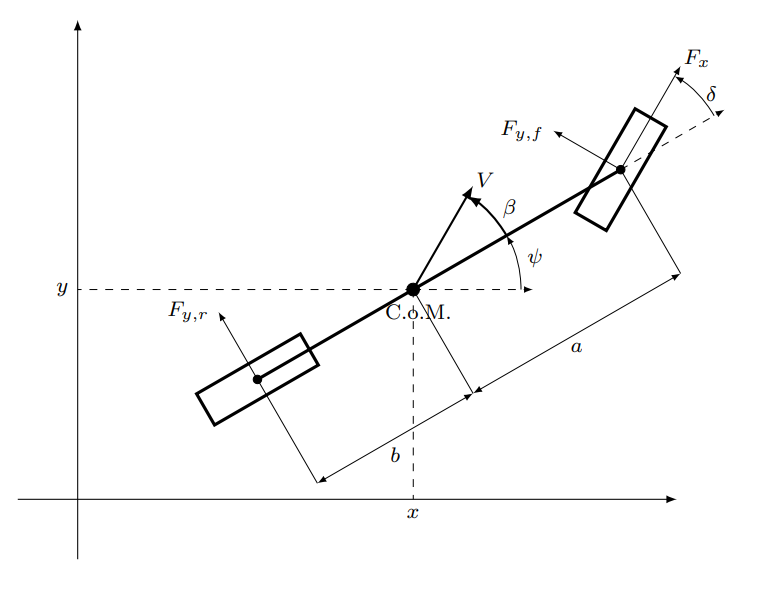
\includegraphics[scale=.40]{figs/Fig1} \\
    \caption{Bicycle model}
    \label{fig:bicycle_model}
\end{figure}
\\
The dynamic model is:
\begin{align*}
\dot x &= V cos \beta cos \psi - V sin \beta sin \psi \\
\dot y &= V cos \beta sin \psi + V sin \beta cos \psi \\
 m \dot V &= F_y,_r sin \beta+F_x cos(\beta - \delta) + F_y,_f sin(\beta - \delta)\\
\dot \beta &= \frac{1}{mV} (F_y,_r cos \beta + F_y,_f cos (\beta-\delta)-F_x sin(\beta-\delta)-\dot\psi)\\
I_z \ddot \psi &= (F_x sin \delta + F_y,_f cos \delta) a - F_y,_r b.
\end{align*}
where:
\begin{itemize}
    \item (x, y, $\psi$) are the cartesian coordinates of the center of mass of the vehicle and its yaw in a global reference frame;
    \item V is the speed modulus in body fixed reference frame;
    \item $\beta$ is the angle between the speed and the body fixed reference frame;
    \item $\dot\psi$ is the yaw rate;
\end{itemize}
\\
\begin{itemize}
    \item $\delta$ is the steering angle of the vehicle;
    \item $F_x$ is the force applied by the front wheel.
\end{itemize}
The lateral forces $F_{y,f}$,$F_{y,r}$  can be found as 
\begin{align*}
    F_y,_f &= \mu F_z,_f \beta_f\\
    F_y,_r &= \mu F_z,_f \beta_r
\end{align*}
\\
where $\beta_f , \beta_r$ are the front and real sideslip angles, 
\begin{align*}
    \beta_f &= \delta - \frac{V sin(\beta) + a \dot \psi}{V cos(\beta)}\\
    \beta_r &= - \frac{V sin(\beta) - b \dot \psi}{V cos(\beta)}
\end{align*}
\\
The vertical forces on the front and rear wheel can be found as: 
\begin{align*}
    F_{z,f} &= \frac{m g b}{a+ b}\\
    F_{z,r} &= \frac{m g a}{a+ b}
\end{align*}
\\
The mechanical parameters of the car are available in Table \ref{param_table}. 
\begin{table}[h]
\begin{center}
\begin{tabular}{c|c c}
\multicolumn{1}{l|}{} & \multicolumn{1}{l}{\textbf{Parameters:}} \\ \hline
$m$                    & $1480$ &$[Kg]$                             \\
$I_z$                    & $1950$ &$[Kgm^2]$                             \\
$a$                    & $1.421$ &$[m]$                             \\
$b$                    & $1.029$ &$[m]$                             \\
$\mu$                    & $1$ &$[nodim]$                             \\
$g$                    & $9.81$ &$[\frac{m}{s^2}]$                             
\end{tabular}
\caption{\label{param_table}Mechanical parameters of the vehicle}
\end{center}
\end{table}

\section{State space and control inputs}
\\Considering the following state space $x=[x,y,\psi,V,\beta,\dot\psi]^T$ and the control input $u=[\delta,F_x]^T$ it's possible to rewrite the dynamics in state-space model:
\begin{align*}
\dot x_1 &= x_4 cos x_5 cos x_3 - x_4 sin x_5 sin x_3 \\
\dot x_2 &= x_4 cos x_5 sin x_3 + x_4 sin x_5 cos x_3 \\
\dot x_3 &= x_6 \\
\dot x_4 &= \frac{F_{y,r} sin x_5+u_2 cos(x_5 - u_1) + F_{y,f} sin(x_5 - u_1)}{m}\\
\dot x_5 &= \frac{1}{m_x_4} (F_{y,r} cos x_5 + F_{y,f} cos (x_5-u_1)-u_2sin(x_5-u_1)-x_6)\\
\dot x_6&= \frac{(u_2 sin u_1 + F_{y,f} cos u_1) a - F_{y,r} b}{I_z}
\end{align*}
To represent the dynamics in the state space, we decide to add a state $x_3$ to avoid deriving $\dot x_5$
at a later time step.  Just to handle the derivation of states in a more appropriate way.

\section{Discretization}
The discrete-time state-space equations were defined using the Forward Euler discretization method, since the algorithm works in discrete time:
\begin{align*}
    x_{1,t+1} &= x_{1,t} + d(x_{4,t} cos x_{5,t} cos x_{3,t} - x_{4,t} sin x_{5,t} sin x_{3,t})\\
    x_{2,t+1} &= x_{2,t} + d(x_{4,t} cos x_{5,t} sin x_{3,t} + x_{4,t} sin x_{5,t} cos x_{3,t})\\
    x_{3,t+1} &= x_6\\
    x_{4,t+1} &= x_{4,t} + d\frac{F_{y,r,t} sin x_{5,t} + u_{2,t} cos(x_{5,t} - u_{1,t}) + F_{y,f,t} sin(x_{5,t} - u_{1,t})}{m}\\
    x_{5,t+1} &= x_{5,t} + d\left(\frac{1}{m x_{4, t}} \left(F_{y, r, t} \cos x_{5,t} + F_{y,f,t} \cos(x_{5,t} - u_{1,t}) - u_{2,t} \sin(x_{5,t} - u_{1,t}) - x_{6,t}\right)\right)\\
    x_{6,t+1} &= x_{6,t} + d\frac{(u_{2,t} sin u_{1,t} + F_{y,f,t} cos u_{1,t})a - F_{y,r,t} b}{I_z}
\end{align*}
Where $d$ is a time interval, usually set to $10^{-3}$.

\section{Dynamics function}
The dynamics function takes as input:
\begin{itemize}
    \item x : state of the system at time t
    \item u : given input for the system
\end{itemize}
\\It mathematically describes how the state variables of the system evolve over time, producing an output that represents the state of the system at the next instant, namely t+1.\\\\
The function \texttt{dynamics()} is located within the file \texttt{dynamics.py}, which, in addition to simulating the dynamics and returning the state at the next time instant, also returns the Jacobians with respect to the states and inputs. The latter are computed for future purposes.\\\\

%%%%%%%%%% Task 1 %%%%%%%%%%
\setcounter{section}{+1}
\chapter{Task 1 - Trajectory generation (I)}\label{chapter:task1}
Compute two equilibria for your system and define a reference curve between the two.
Compute the optimal transition to move from one equilibrium to another exploiting the Newton's-like algorithm for optimal control.

\section{Equilibrium Computation}
To compute the equilibria, the derivatives of the system have been set to zero:
\begin{center}
    x_{1,t+1} - x_{1,t} - d(x_{4,t} cos x_{5,t} cos x_{3,t} - x_{4,t} sin x_{5,t} sin x_{3,t}) &= 0\\
    x_{2,t+1} - x_{2,t} - d(x_{4,t} cos x_{5,t} sin x_{3,t} + x_{4,t} sin x_{5,t} cos x_{3,t}) &= 0\\
    x_{3,t+1} - x_6 &= 0 \\
    x_{4,t+1} - x_{4,t} - d\frac{F_{y,r,t} sin x_{5,t} + u_{2,t} cos(x_{5,t} - u_{1,t}) + F_{y,f,t} sin (x_{5,t} - u_{1,t})}{m} &= 0\\
    x_{5,t+1} - x_{5, t} - d\left(\frac{1}{m x_{4, t}} \left(F_{y, r, t} \cos x_{5, t} + F_{y, f, t} \cos(x_{5, t} - u_{1, t}) - u_{2, t} \sin(x_{5, t} - u_{1, t}) - x_{6, t}\right)\right) &= 0\\
    x_{6,t+1} - x_{6,t} - d\frac{(u_{2,t} sin u_{1,t} + F_{y,f,t} cos u_{1,t})a - F_{y,r,t} b}{I_z} &= 0\\
\end{center}
When solving this system it was deemed appropriate to focus on one of the possible configurations:
\begin{center}
    x_1 = 0\\
    x_2 = 0\\
    x_3 = 0\\
    x_4 = \widetilde{x_4}\\
    x_5 = 0\\
    x_6 = 0\\
    u_1 = 0\\
    u_2 = 0\\
\end{center}
$x_4 = \widetilde{x_4}$ denotes a constant value.\\
Therefore the following two equilibria were chosen:
\begin{center}
    x_{1,e} = [0, 0, 0, 10, 0, 0]^T\\
    x_{2,e} = [0, 0, 0, 20, 0, 0]^T\\
    u_{1,e} = u_{2,e} = [0, 0]^T\\
\end{center}

\section{Reference curve definition}
The reference curve was chosen in such a way as to pass from the equilibrium $(x_{1,e}, u_{1,e})$ to the equilibrium $(x_{2,e}, u_{2,e})$.\\
In particular, considering a time interval of 10 seconds, the system maintains a constant speed of $10\;m/s$ for the first 5 seconds and then switches to a constant speed of $20\;m/s$ for the remaining 5 seconds, as shown in \ref{fig:ref_x4_task1}:
\begin{figure}[h]
    \centering
    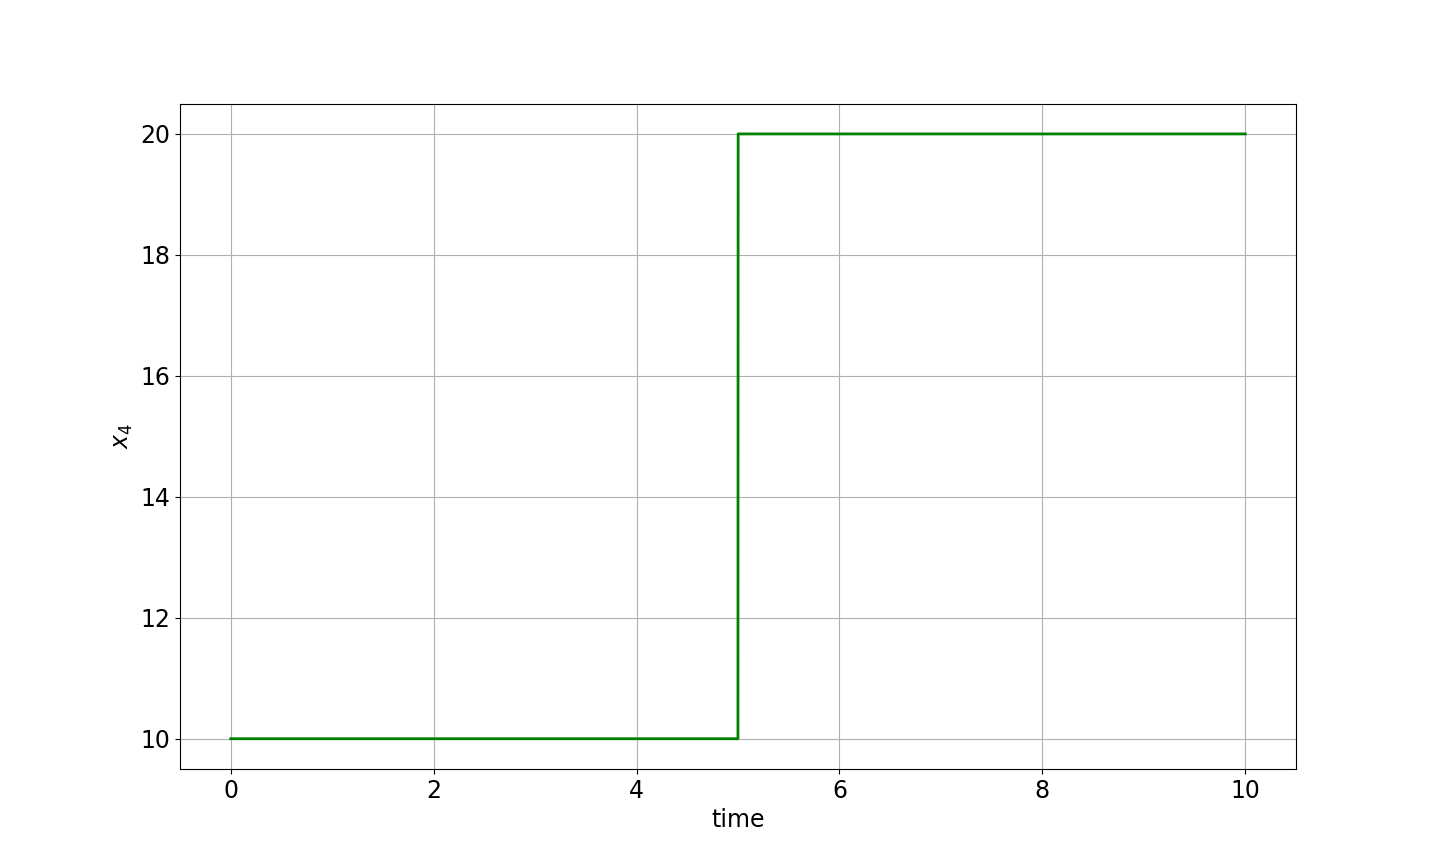
\includegraphics[scale=.28]{figs/Task1/ref_x4} \\
    \caption{Reference curve}
    \label{fig:ref_x4_task1}
\end{figure}
\\
Instead, the position ($x_1$ and $x_2$) was calculated by forward integrating the dynamics for the first 5 seconds with the values of the first equilibrium $(x_{1,e}, u_{1,e})$ and for the following 5 seconds with the values of the second equilibrium $(x_{2,e}, u_{2,e})$. Therefore the reference curve defined is shown in the plot of Figure \ref{fig:ref_curve_task1}.\\
\begin{figure}[h]
    \centering
    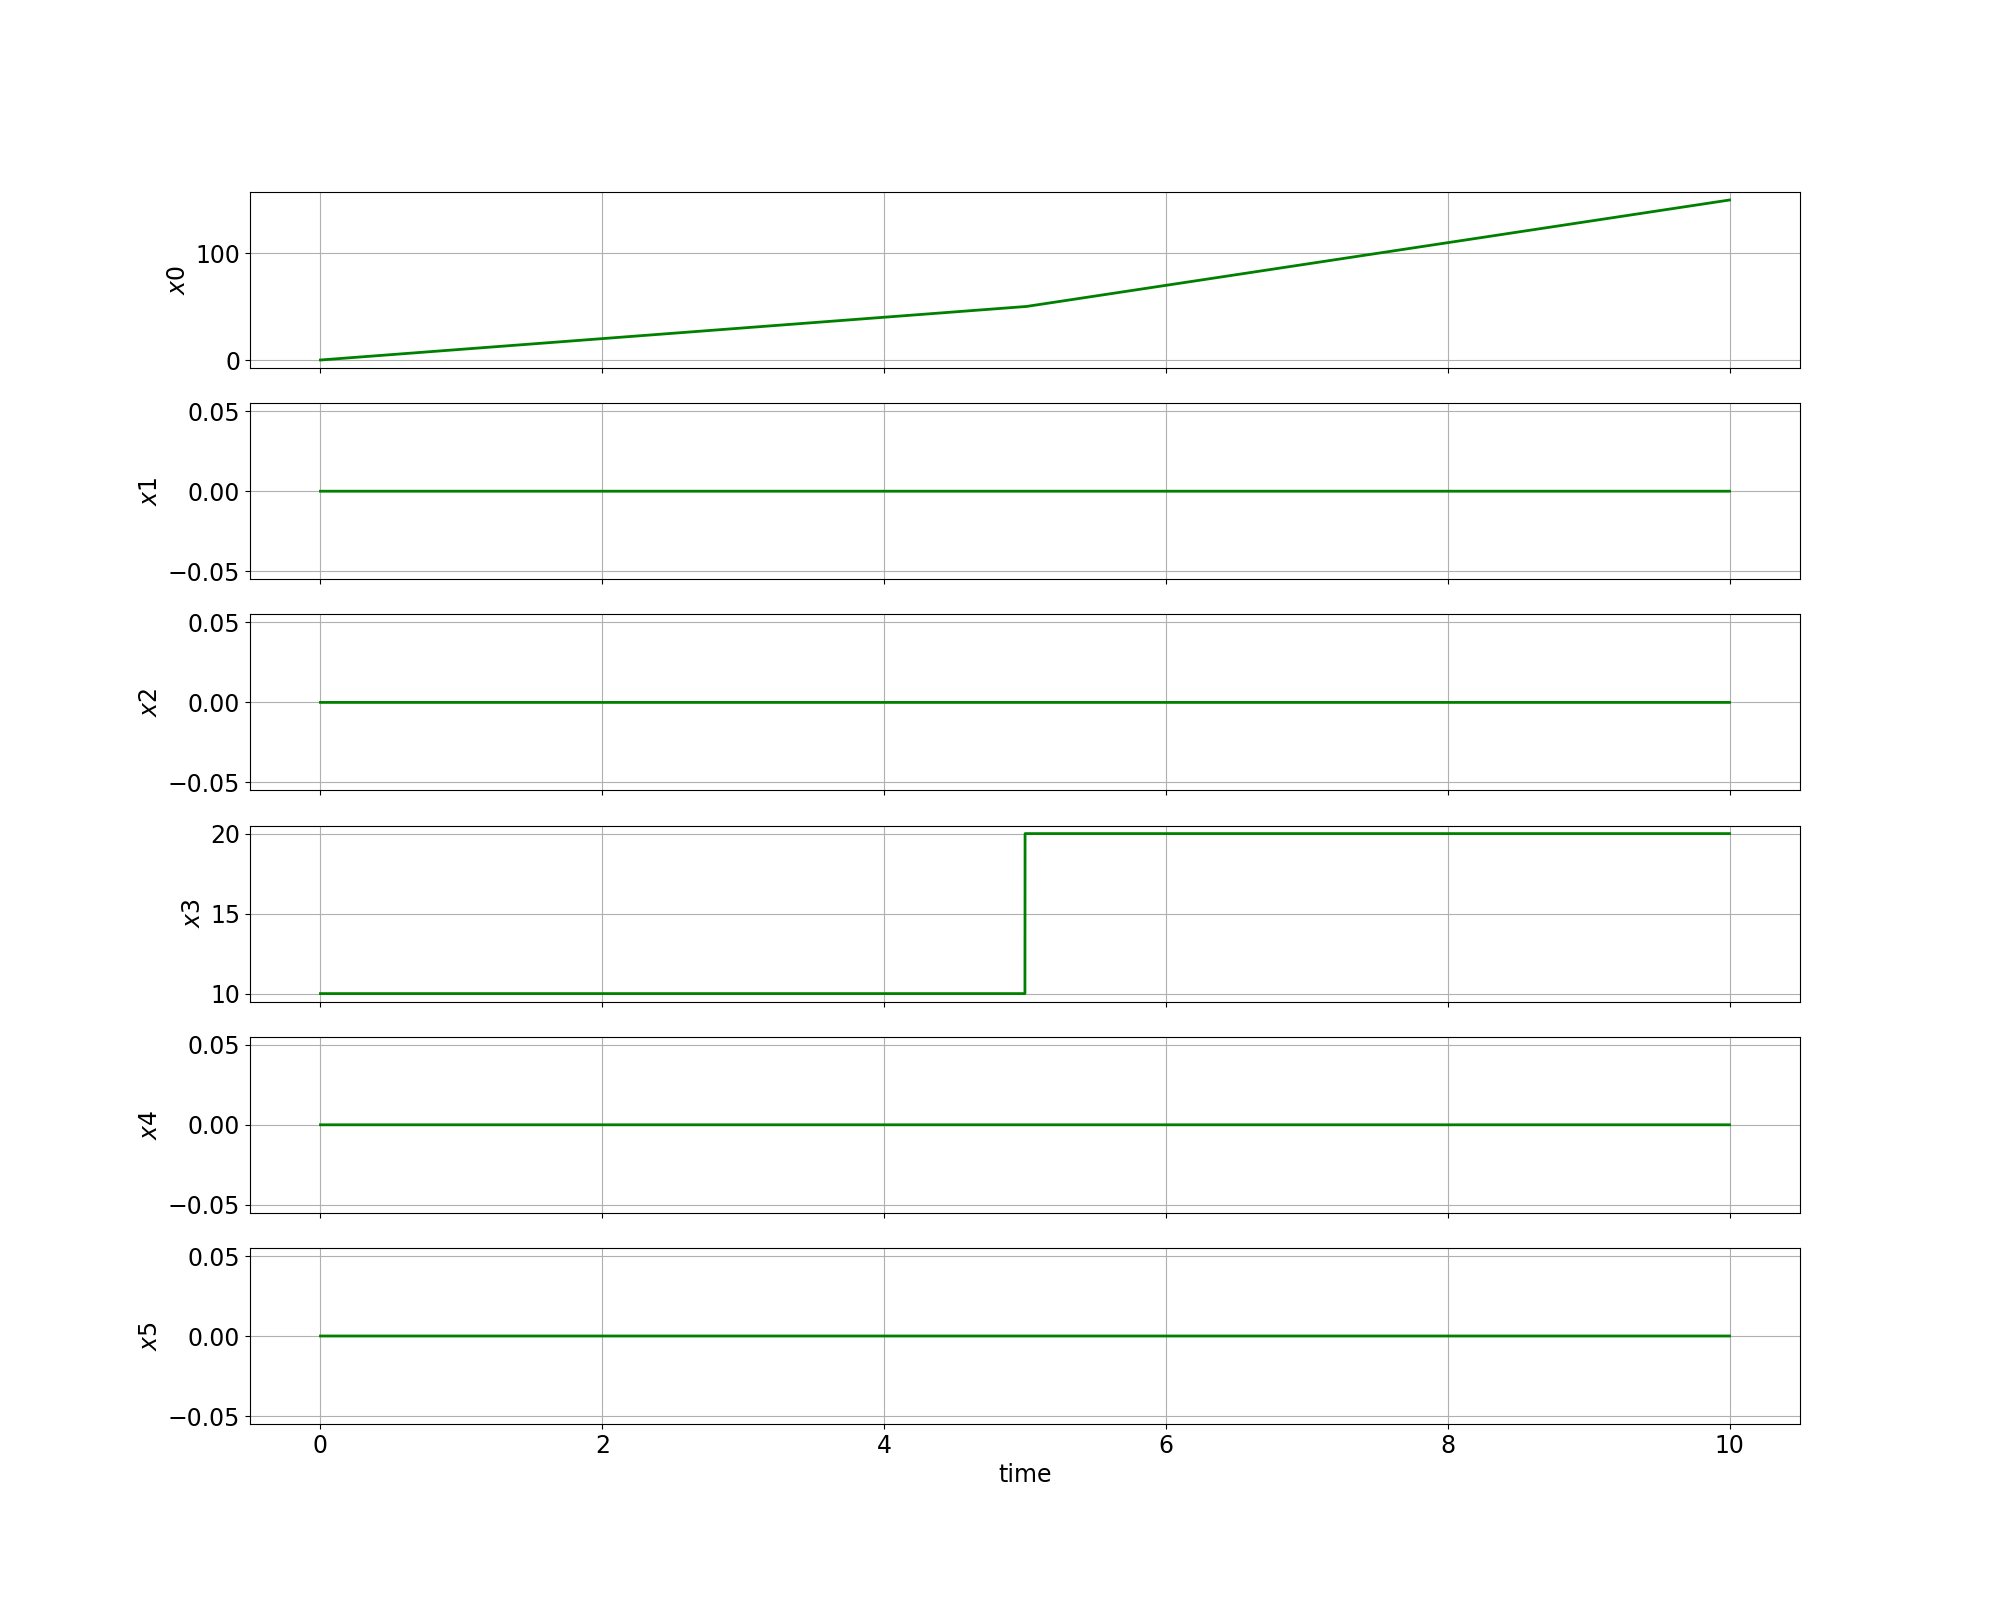
\includegraphics[scale=.25]{figs/Task1/ref_curve} \\
    \caption{Reference curve}
    \label{fig:ref_curve_task1}
\end{figure}
\newpage
\section{Linear Quadratic Regularization}
To solve the optimal control problem it's been implemented Linear Quadratic Regularization (LQR).
\subsection{Newton's method implementation}
\textbf{Initialization}\\
Consider as initial guess trajectory the first equilibrium point $(x_0, u_0)$.\\
For $k$ = 0, 1, . . .:\\

\textbf{Step 1: Compute Descent Direction}\\

Linearize the system dynamics evaluating\\
\begin{align*}
\nabla_1 f_t(x_k^t, u_k^t), \nabla_2 f_t(x_k^t,u_k^t),\nabla_1l_t(x_k^t),\nabla_2l_t(x_k^t,u_k^t),\nablal_T(x_k^T)\\
\end{align*}

Compute the gradient of the reduced cost solving backwards the co-state equation, with

$\lambda_k^T=\nabla l_T(x_k^T)$, and compute $Q_k^t,R_k^t,S_k^t,$ and $Q_k^T$.

In order to define the LQR controller compute $K_k^t,\sigma_k^t,$ for all t = 0,...,T-1:\\
\begin{align*}
    \min_{\Delta x,\Delta u} \sum_{t=0}^{T-1}&
    \begin{bmatrix}
    \nabla_1 l_t(x_k^t,u_k^t\\
    \nabla_2 l_t(x_k^t,u_k^t)\Delta u_t
    \end{bmatrix}^T
    \begin{bmatrix}
           \Delta x_t \\
           \Delta u_t \\ 
           \end{bmatrix}\\
    &+\frac{1}{2}\begin{bmatrix}
           \Delta x_t \\
           \Delta u_t \\ 
           \end{bmatrix}^T
    \begin{bmatrix}
    Q_k^t & S_k^t,^T\\
    S_k^t & R_k^t
    \end{bmatrix}
    \begin{bmatrix}
           \Delta x_t \\
           \Delta u_t \\ 
           \end{bmatrix}\\
    &+\Delta l_T(x_k^T)^T \Delta_x_T+\frac{1}{2}\Delta x_T^T Q_k^T \Delta x_T\\
\end{align*}

\textbf{Step 2:} Compute new state-input trajectory implementing step-size selection rule, e.g., 

Armijo.

Forward integrate (closed-loop), for all $t=0,...,T-1,$, with $x_0^{k+1} = x_{init}$\\
\begin{center}
    $u_t^{k+1} = u_t^k + K_t^k(x_t^{k+1} - x_t^k) + \gamma^k\sigma_t^k$\\
    $x_{t+1}^{k+1} = f_t(x_t^{k+1},u_t^{k+1})$\\
\end{center}

\subsection{Costs definition}
As can be seen from the following matrices, it was decided to give more weight to the speed and less weight to the force applied by the front wheel.
In this case it was decided to keep the same cost also for the final cost.\\
\begin{center}
    $Q_t$ = \begin{bmatrix}
                1 & 0 & 0 & 0 & 0 & 0\\
                0 & 1 & 0 & 0 & 0 & 0\\
                0 & 0 & 1 & 0 & 0 & 0\\
                0 & 0 & 0 & 10000 & 0 & 0\\
                0 & 0 & 0 & 0 & 1 & 0\\
                0 & 0 & 0 & 0 & 0 & 1\\
            \end{bmatrix}
    $R_t$ = \begin{bmatrix}
                1 & 0\\
                0 & 0.0001\\
            \end{bmatrix}
    $Q_T$ = $Q_t$
\end{center}

\section{Results}
\subsection{Optimal Trajectory}
\begin{figure}[h]
        \centering
        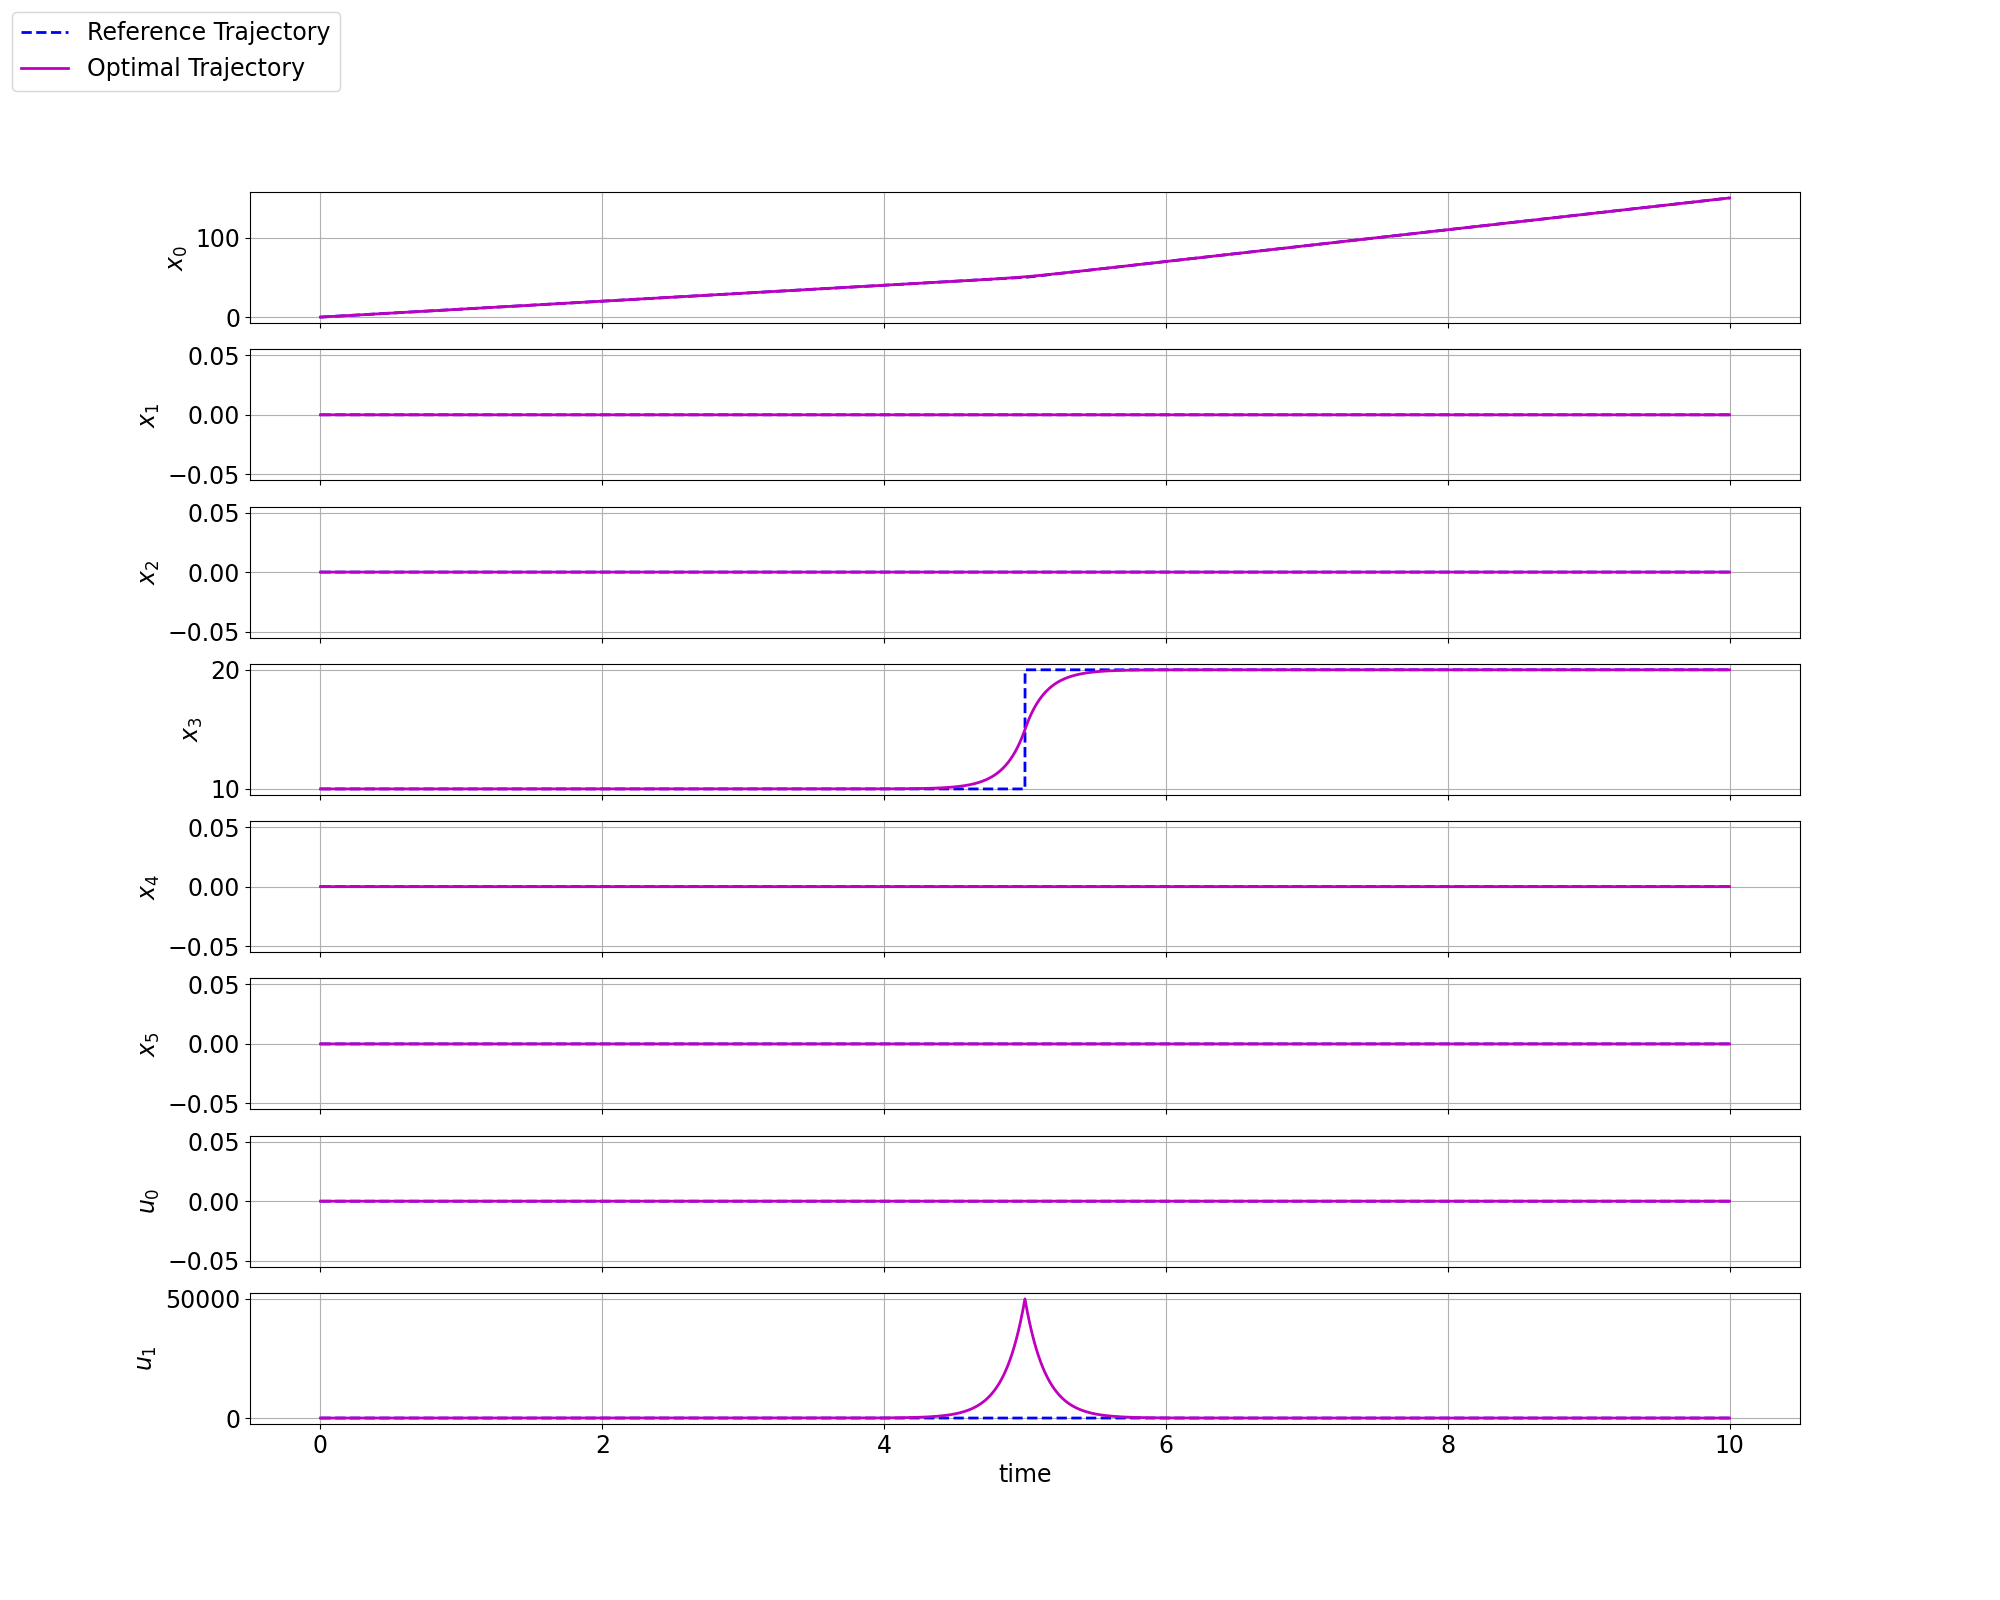
\includegraphics[scale=.32]{figs/Task1/opt_trajectory}
        \caption{Optimal trajectory's plot}
        \label{fig:enter-label}
\end{figure}
\newpage
\subsection{Armijo}
As can be seen from Figure \ref{fig:Armijo's plot iteration 0} and Figure \ref{fig:Armijo's plot iteration 1}, the algorithm converges to the optimal trajectory after just one iteration.

\begin{figure}[h]
    \centering
    \includegraphics[scale=.20]{Report_OPTCON_Project/figs/Task1/armijo_plot_0.png}
    \caption{Armijo's plot iteration 0}
    \label{fig:Armijo's plot iteration 0}
\end{figure}
\begin{figure}[h]
    \centering
    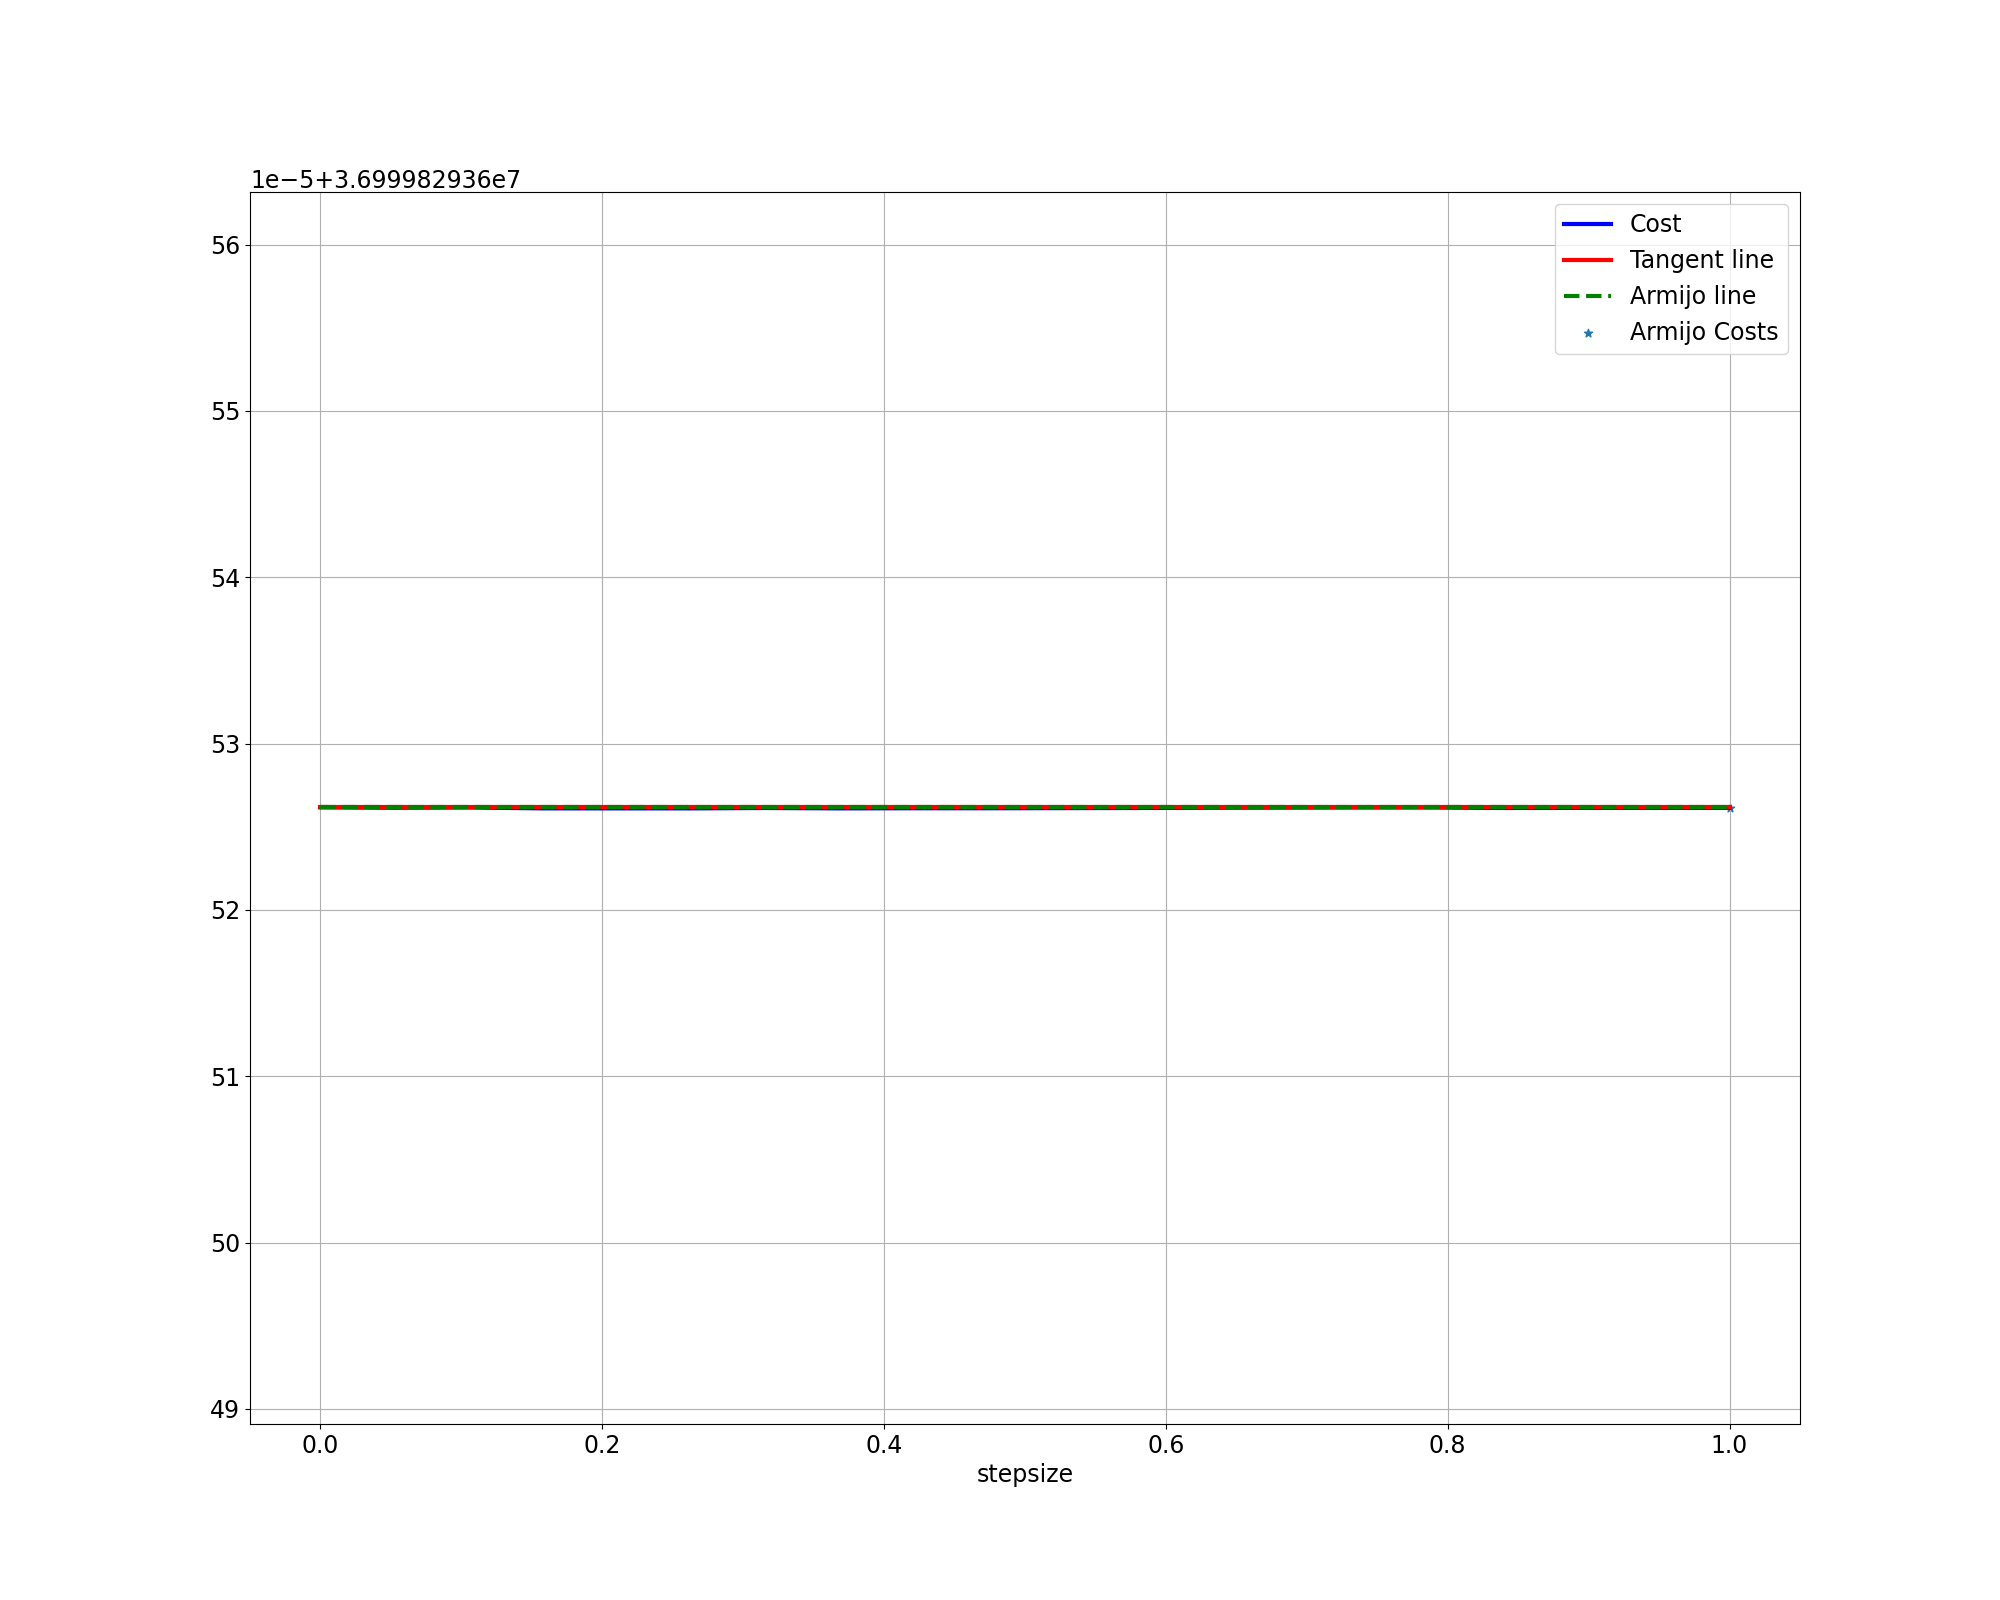
\includegraphics[scale=.20]{Report_OPTCON_Project/figs/Task1/armijo_plot_1.png}
    \caption{Armijo's plot iteration 1}
    \label{fig:Armijo's plot iteration 1}
\end{figure}
\newpage
\newpage

\subsection{Cost and descent direction}
Following the execution, the plots related to the cost and direction generated are displayed.

\begin{figure}[!ht]
    \centering
    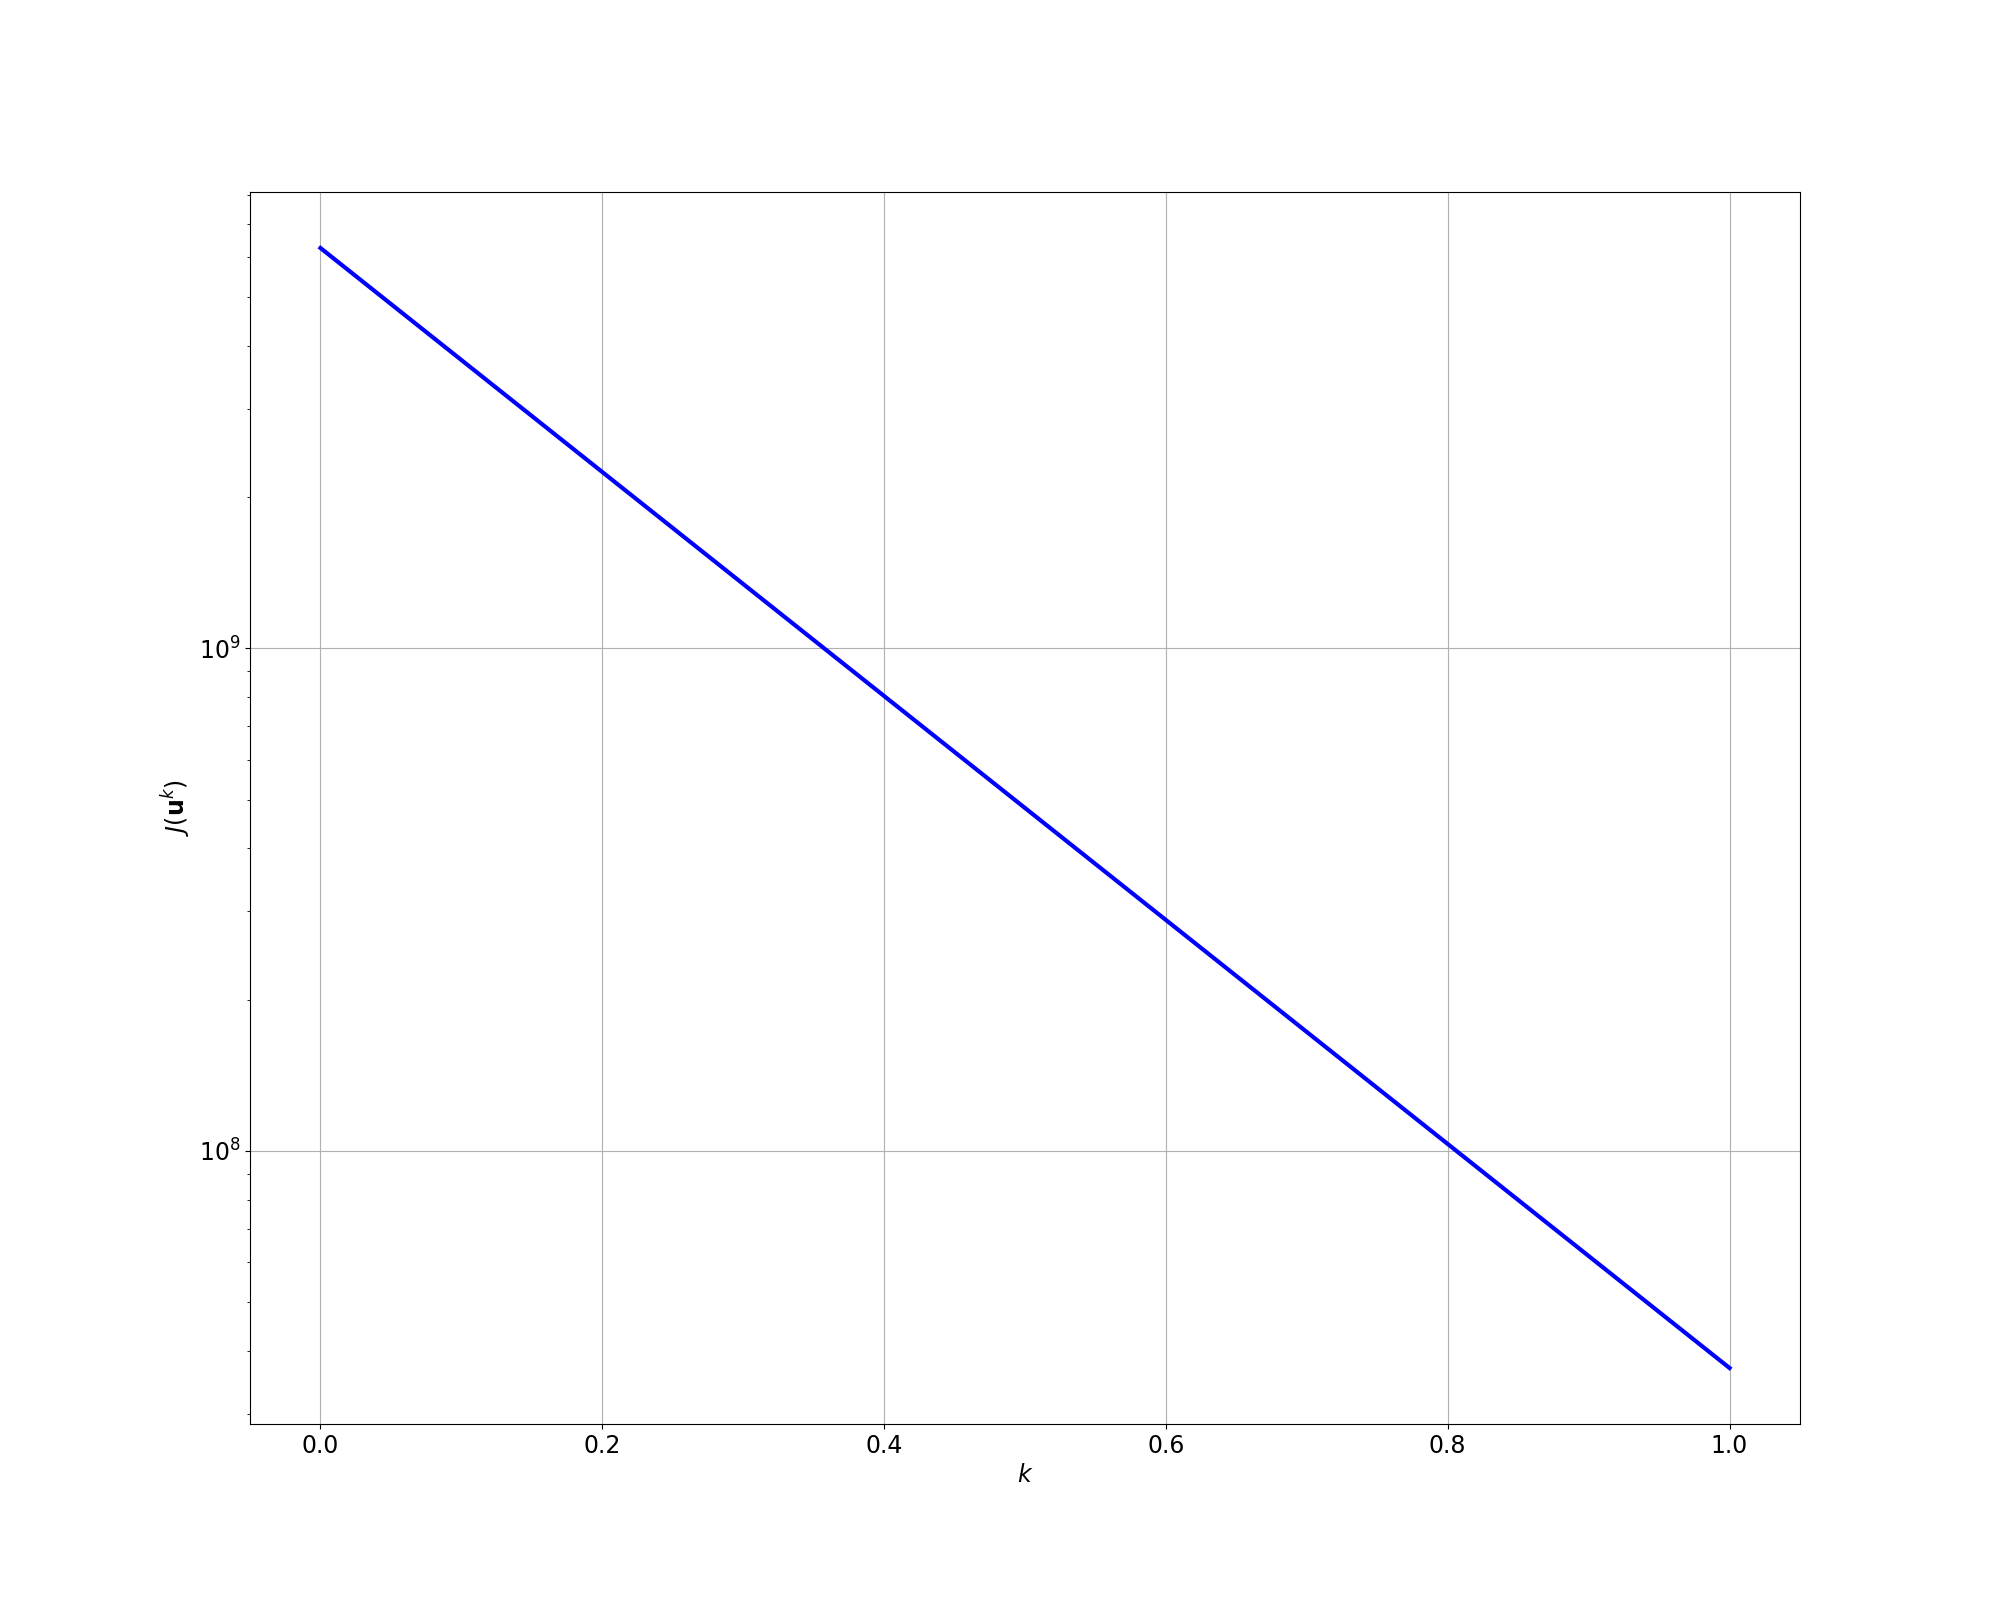
\includegraphics[scale=.20]{figs/Task1/cost}
    \caption{Cost's plot}
    \label{fig:cost}
\end{figure}
\begin{figure}[!ht]
    \centering
    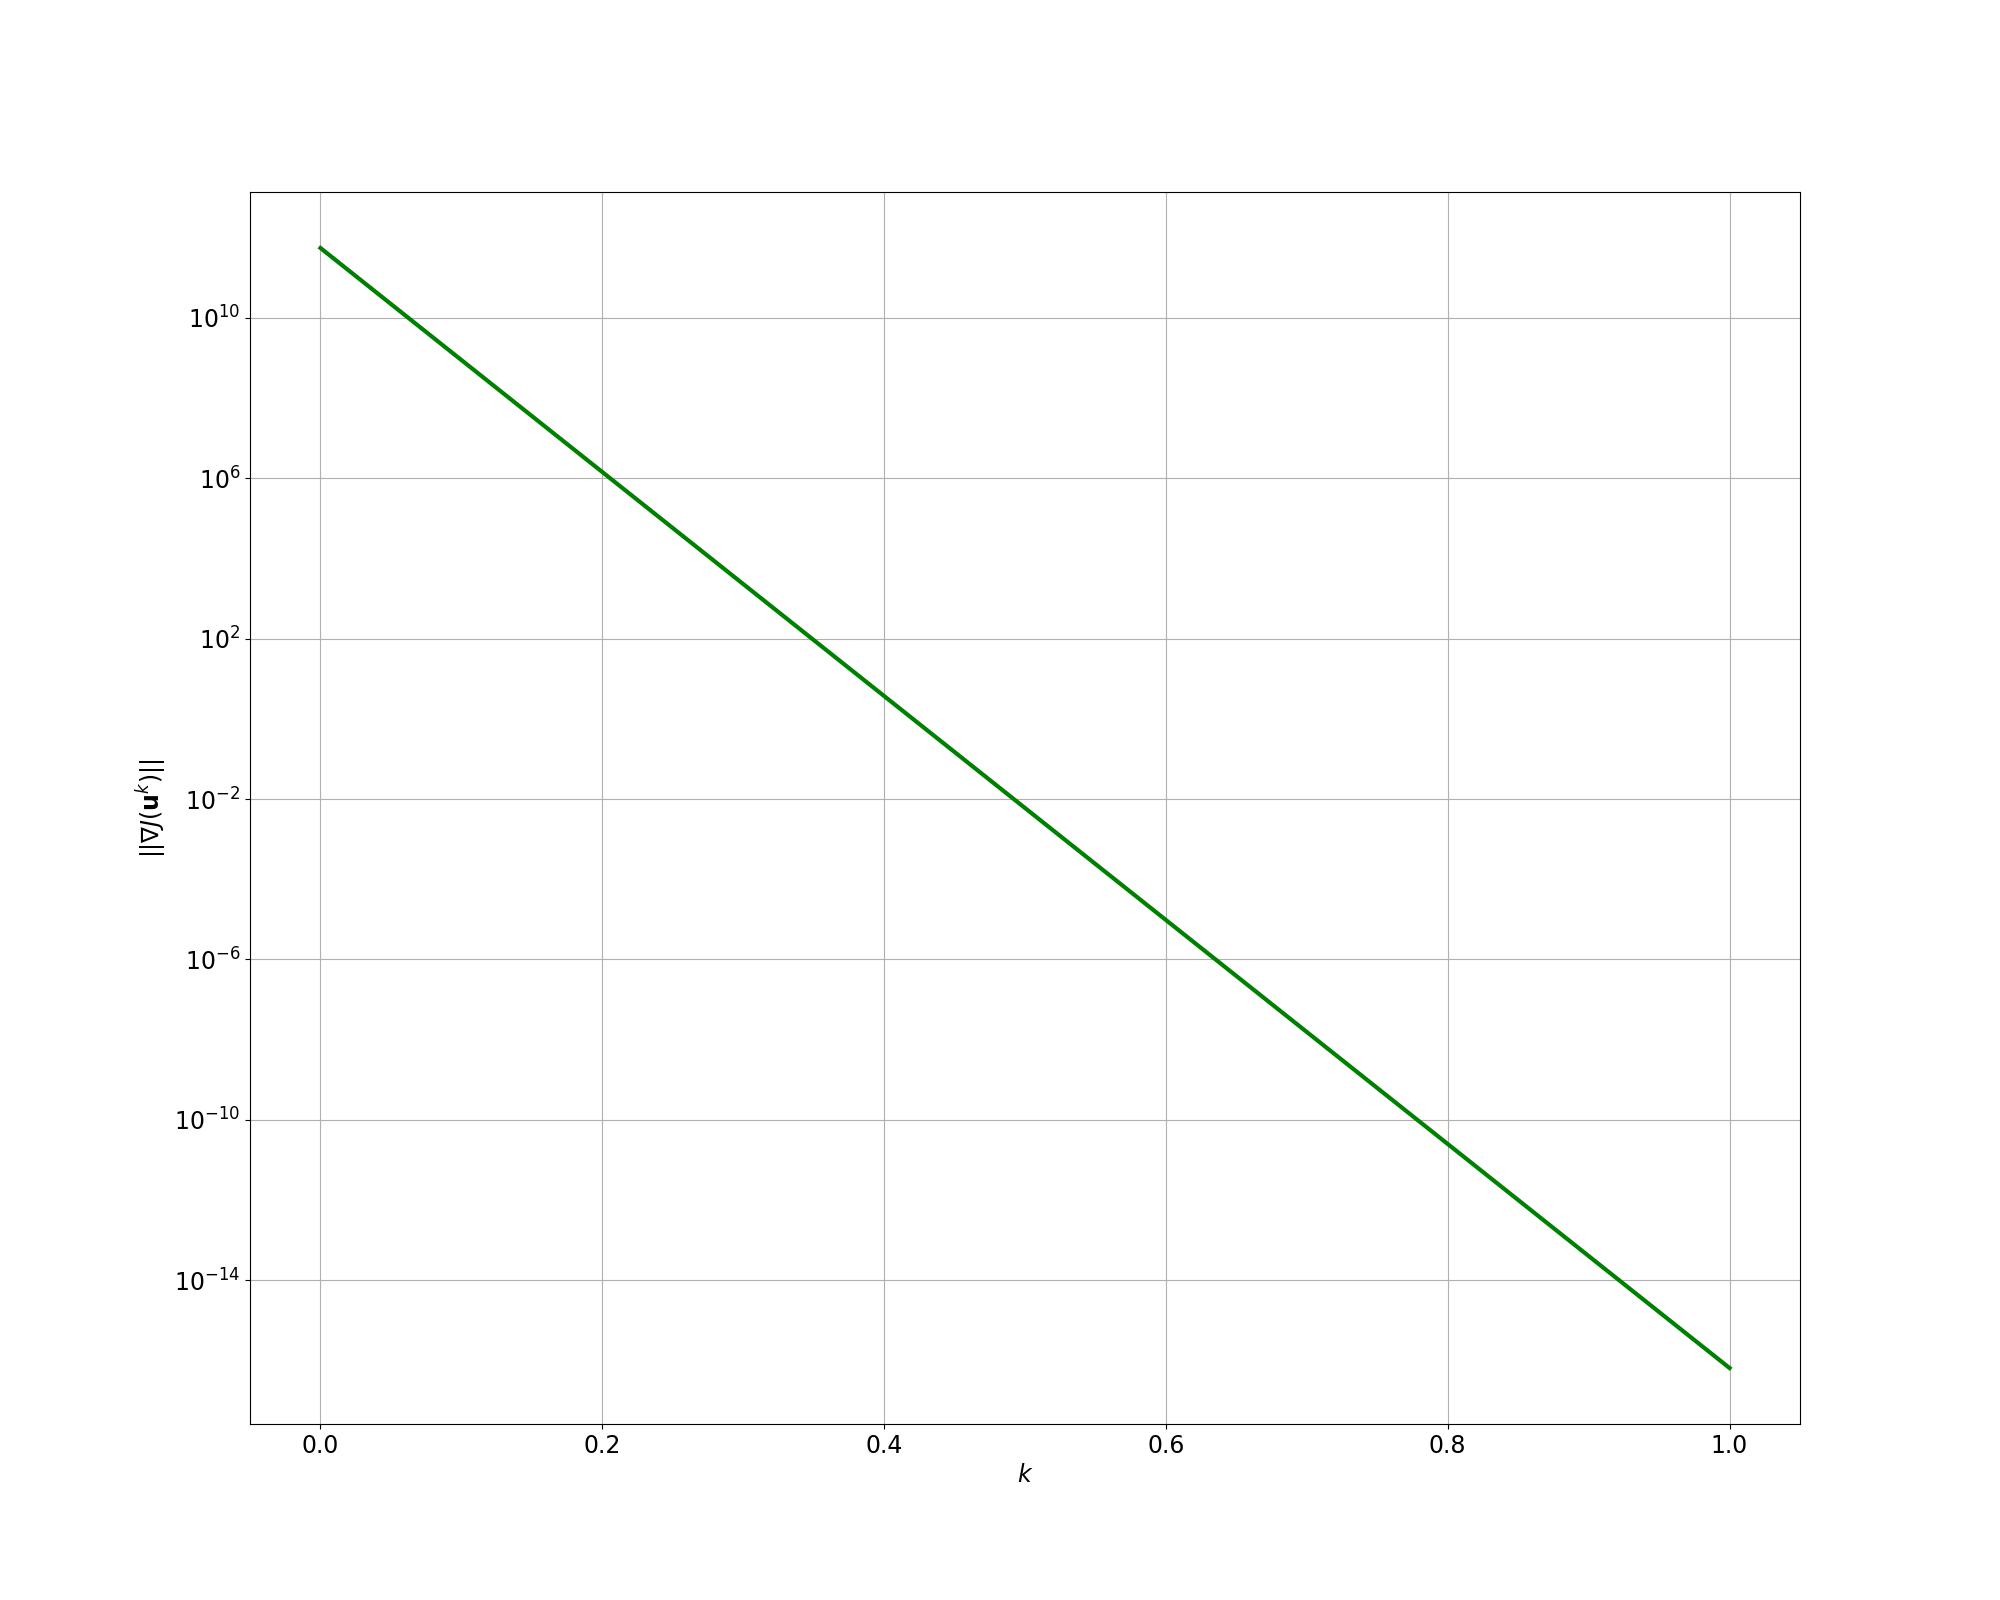
\includegraphics[scale=.20]{figs/Task1/descent_direction}
    \caption{Descent direction's plot}
    \label{fig:desc_dir}
\end{figure}

%%%%%%%%%% Task 2 %%%%%%%%%%
\chapter{Task 2 - Trajectory generation (II)}\label{chapter:task2}
Generate a desired (smooth) state-input curve and perform the trajectory generation task (chapter \ref{chapter:task1}) on this new desired trajectory.\\

\section{Reference curve definition}
In task 2 it's required to generate a desired state-input curve and perform the trajectory generation task of Task 1 (chapter \ref{chapter:task1}) on this new desired trajectory.
In order to generate a smooth state-input curve we opted for a sigmoid trajectory that starts on the first equilibrium state and finishes on the second one. The idea is to change the vehicle's lane while the speed stays constant.\\
The sigmoid function, often denoted as $\sigma(x)$, is defined as:\\
\begin{center}
$\sigma(x)= \frac{1}{1-e^-^x}$\\  
\end{center}
\begin{figure}[h]
    \centering
    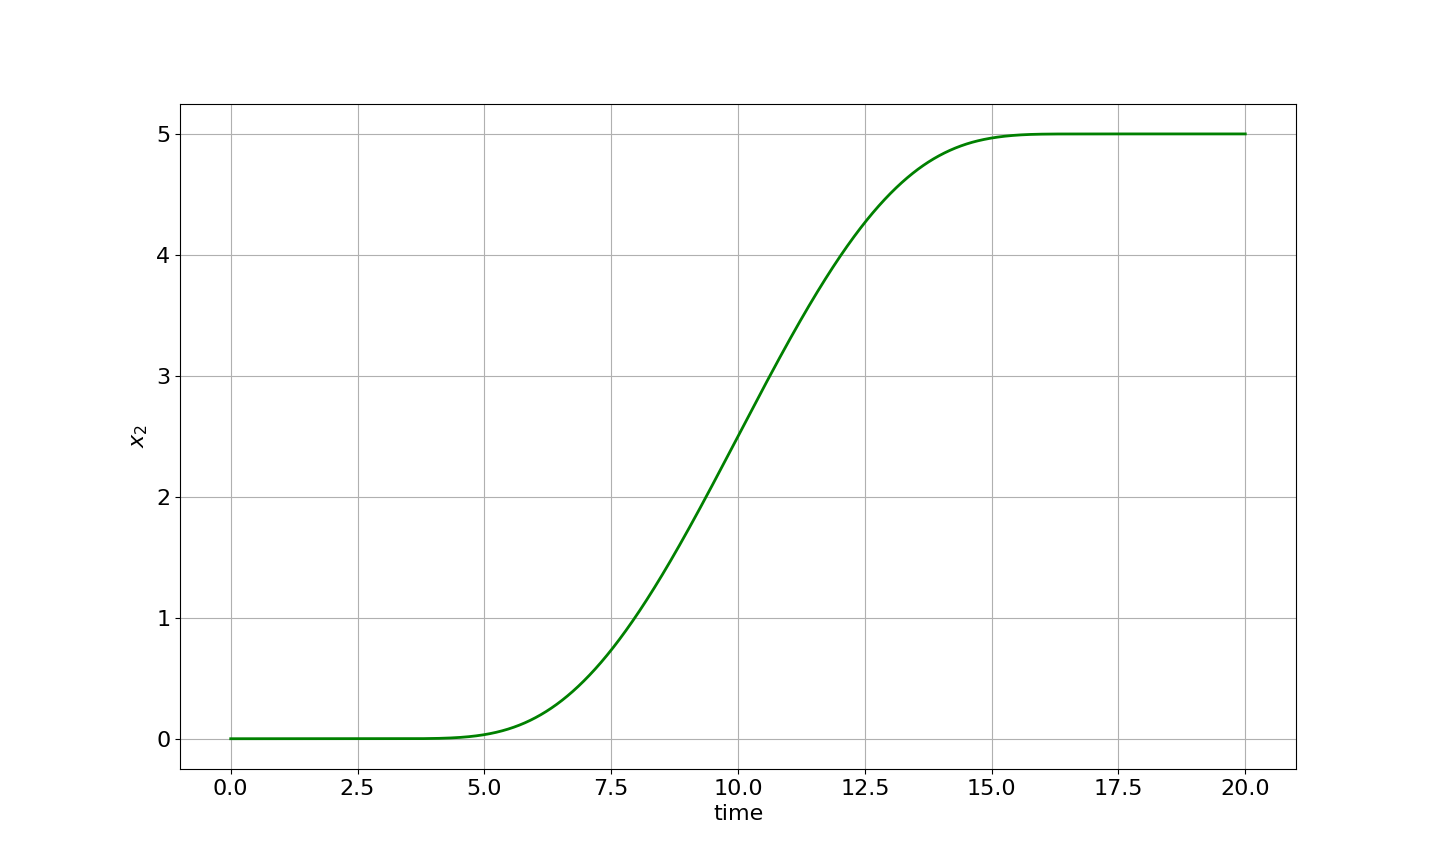
\includegraphics[scale=.27]{figs/Task2/ref_x2}
    \caption{Reference curve's plot}
    \label{fig:enter-label}
\end{figure}

\begin{figure}[h]
    \centering
    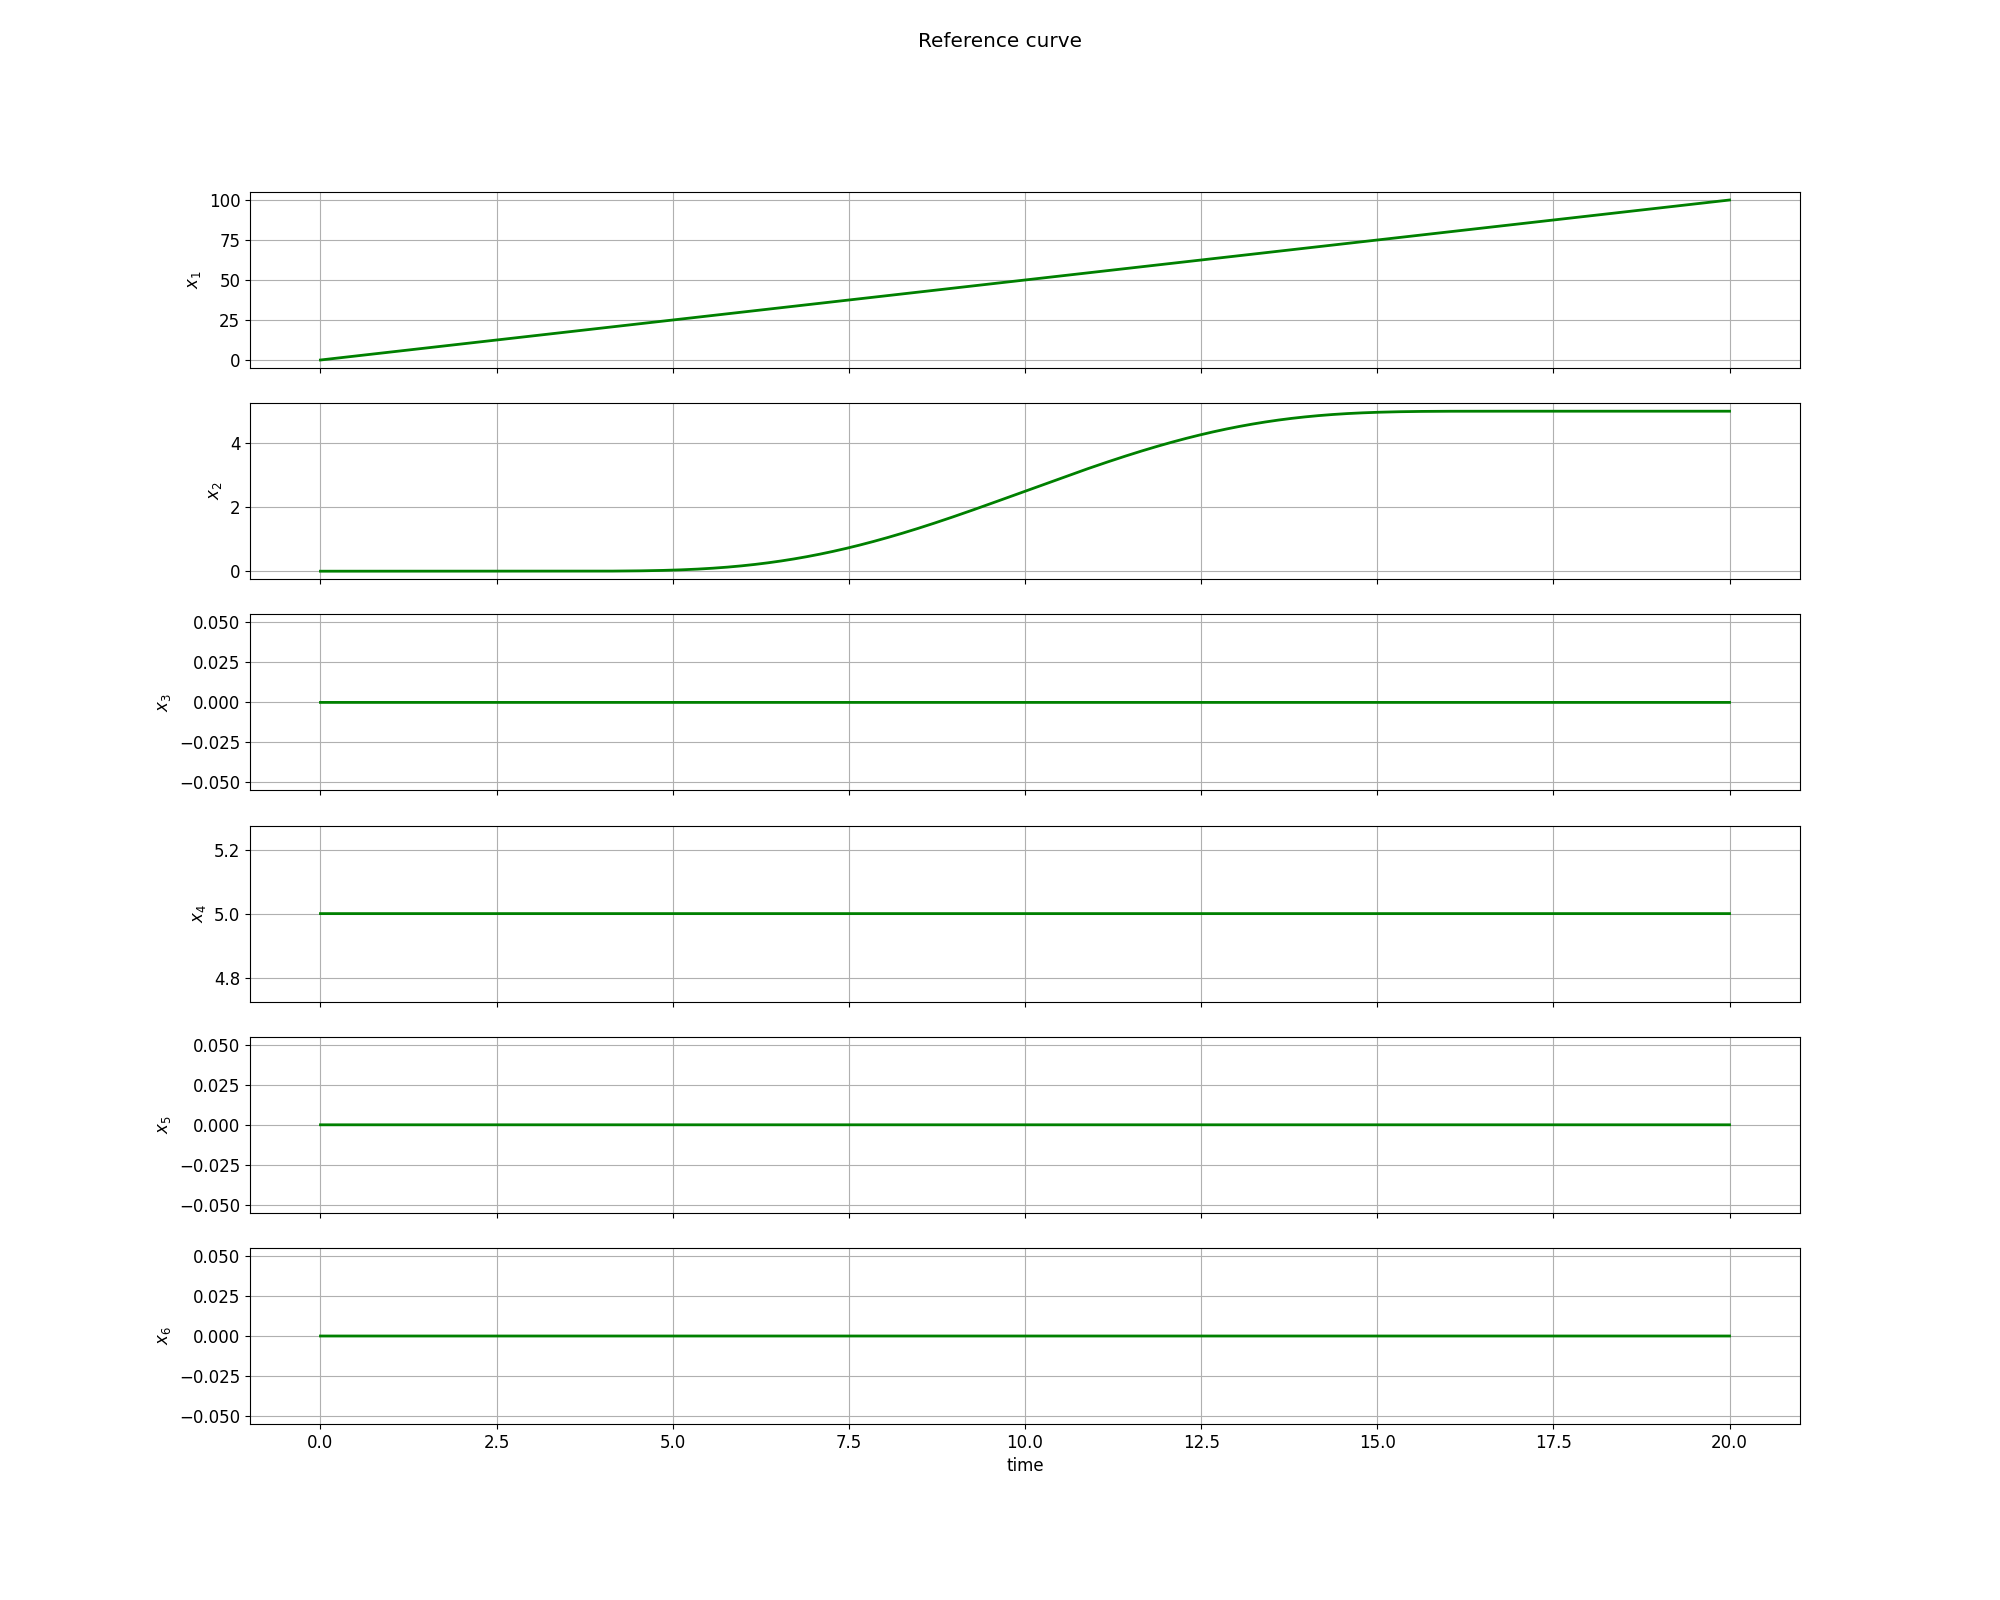
\includegraphics[scale=.3]{figs/Task2/ref_curve.png}
    \caption{Reference curve's plot}
    \label{fig:enter-label}
\end{figure}
\newpage
\section{Linear Quadratic Regularization}
\subsection{Costs definition}
Below are reported the matrices representing the costs.\\
The values contained within have been defined following a weighted choice, considering more weight on $x_1(y)$ and on $u_1(\delta)$, less importance on $u_2(F_x)$ instead.
\begin{center}
    $Q_t$ = \begin{bmatrix}
                100 & 0 & 0 & 0 & 0 & 0\\
                0 & 1000 & 0 & 0 & 0 & 0\\
                0 & 0 & 10 & 0 & 0 & 0\\
                0 & 0 & 0 & 100 & 0 & 0\\
                0 & 0 & 0 & 0 & 100 & 0\\
                0 & 0 & 0 & 0 & 0 & 10\\
            \end{bmatrix}
    $R_t$ = \begin{bmatrix}
                10000 & 0\\
                0 & 0.0001\\
            \end{bmatrix}
\end{center}
$Q_T$ was chosen equal to the solution of the Riccati equation calculated for $A_T$ and $B_T$, which represent the dynamics of the linearized system at instant T.
 \newpage
\section{Results}
\subsection{Optimal Trajectory}
\begin{figure}[h]
    \centering
    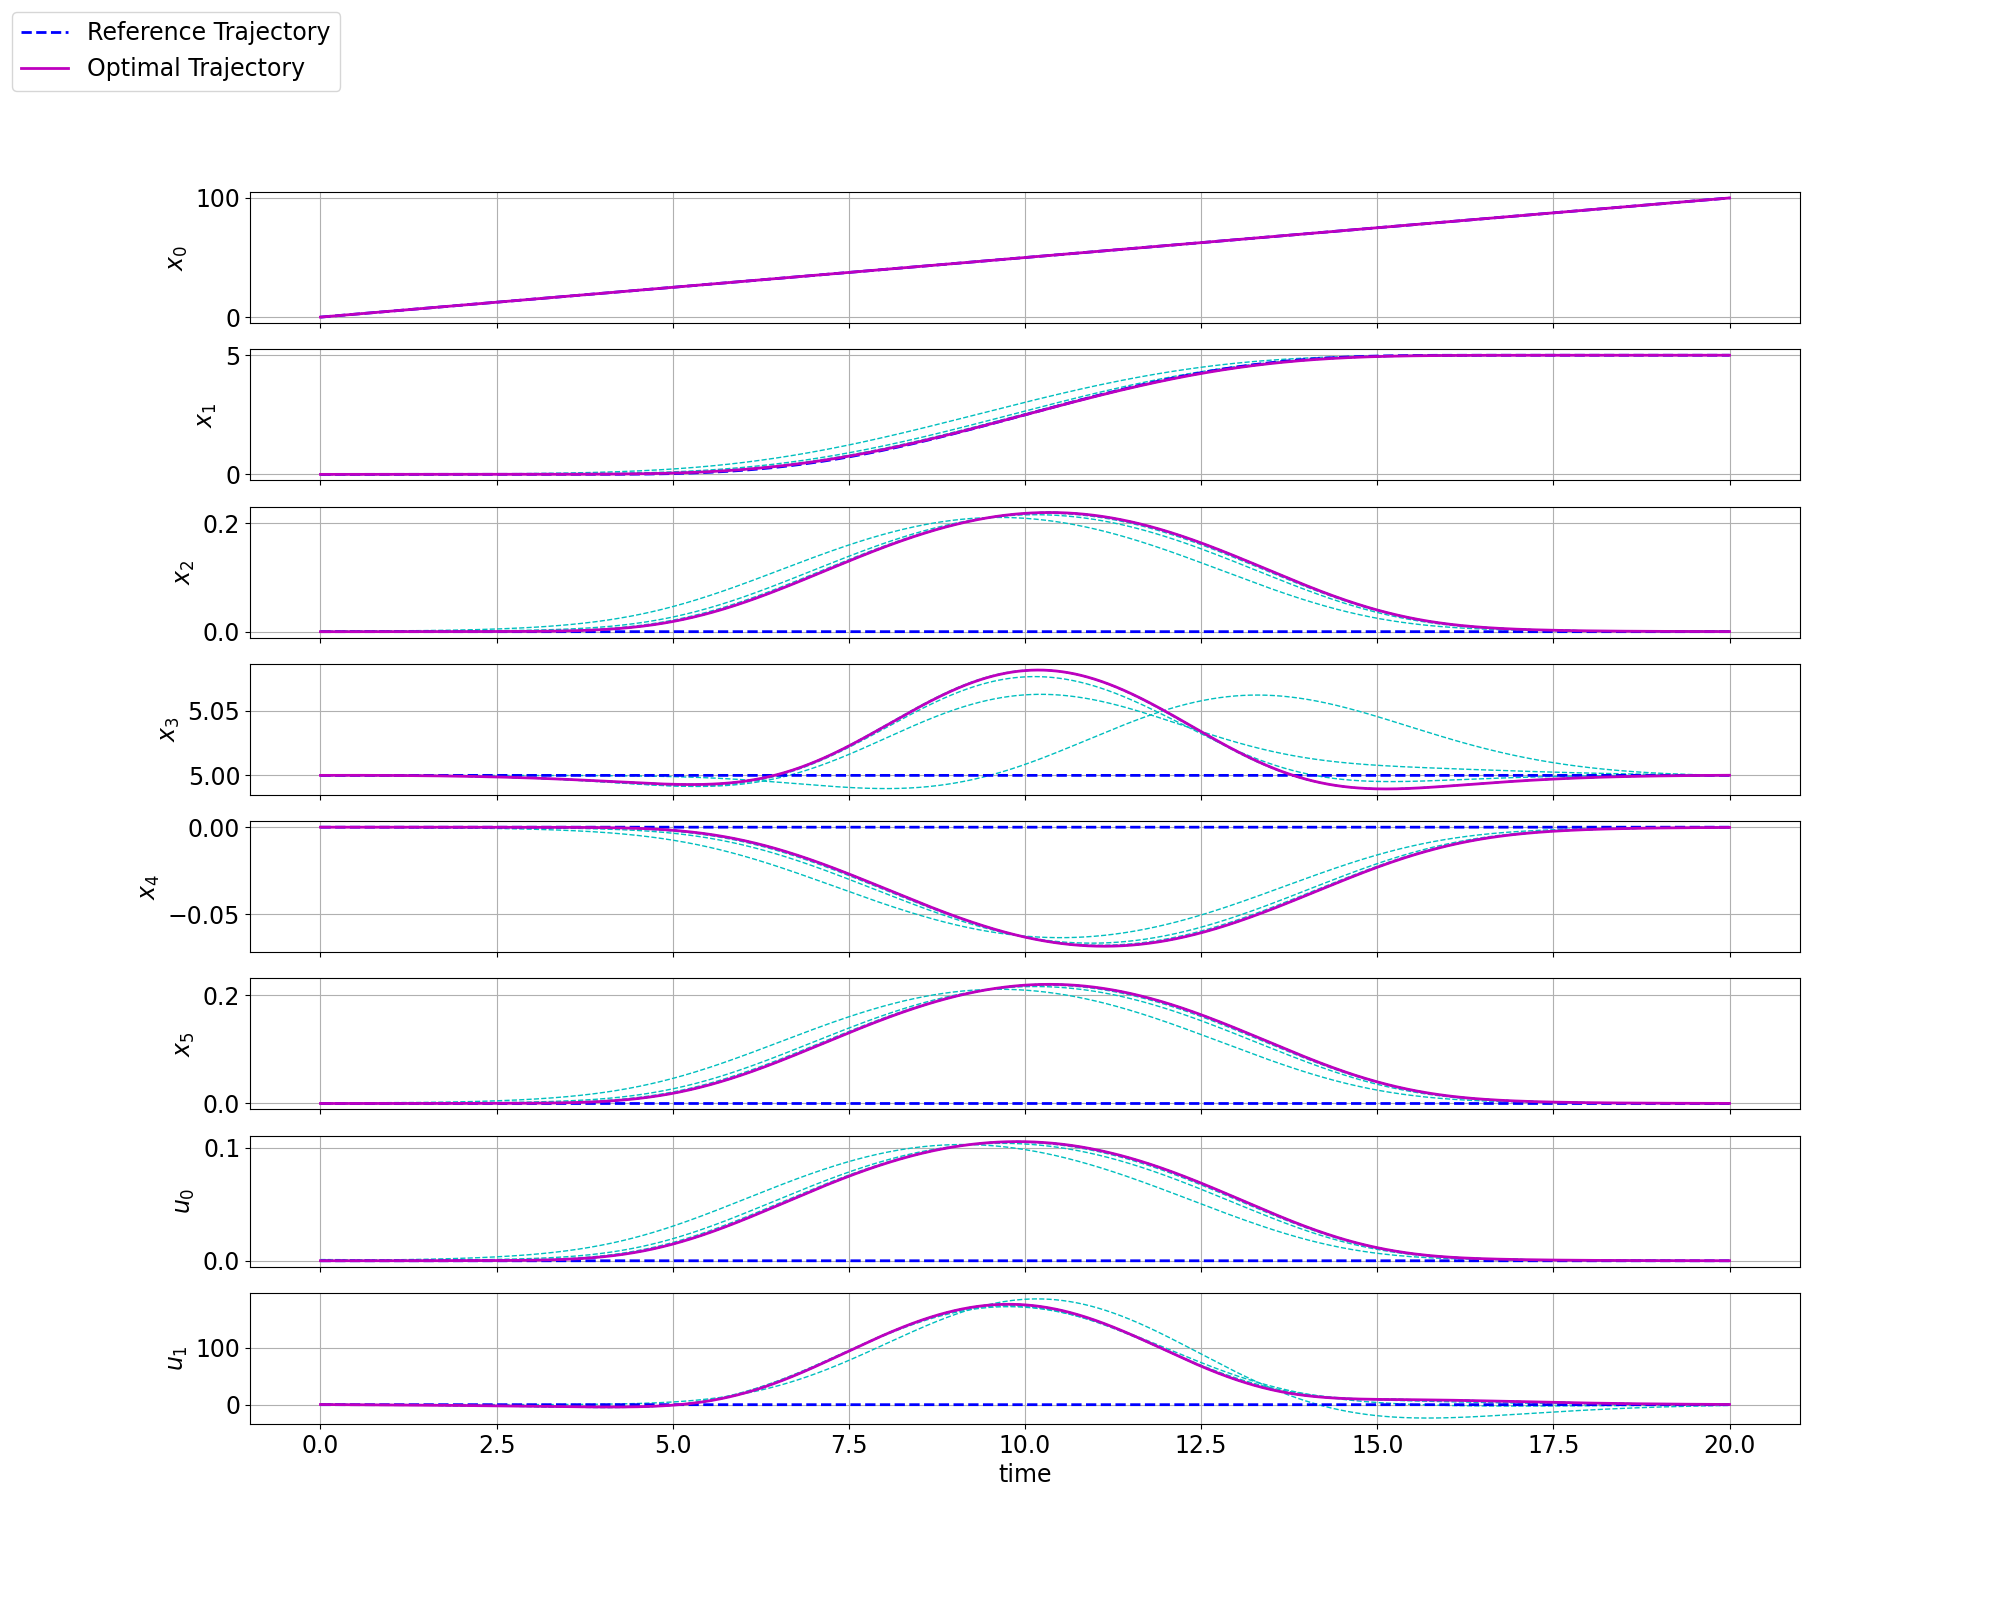
\includegraphics[scale=.3]{Report_OPTCON_Project/figs/Task2/opt_trajectory.png} \\
    \caption{Optimal trajectory's plot}
    \label{fig:optimal-label}
\end{figure}
\newpage
\subsection{Cost and descent direction}
Following the execution of Task 3, the plots related to the cost and direction generated are displayed.
\begin{figure}[h]
    \centering
    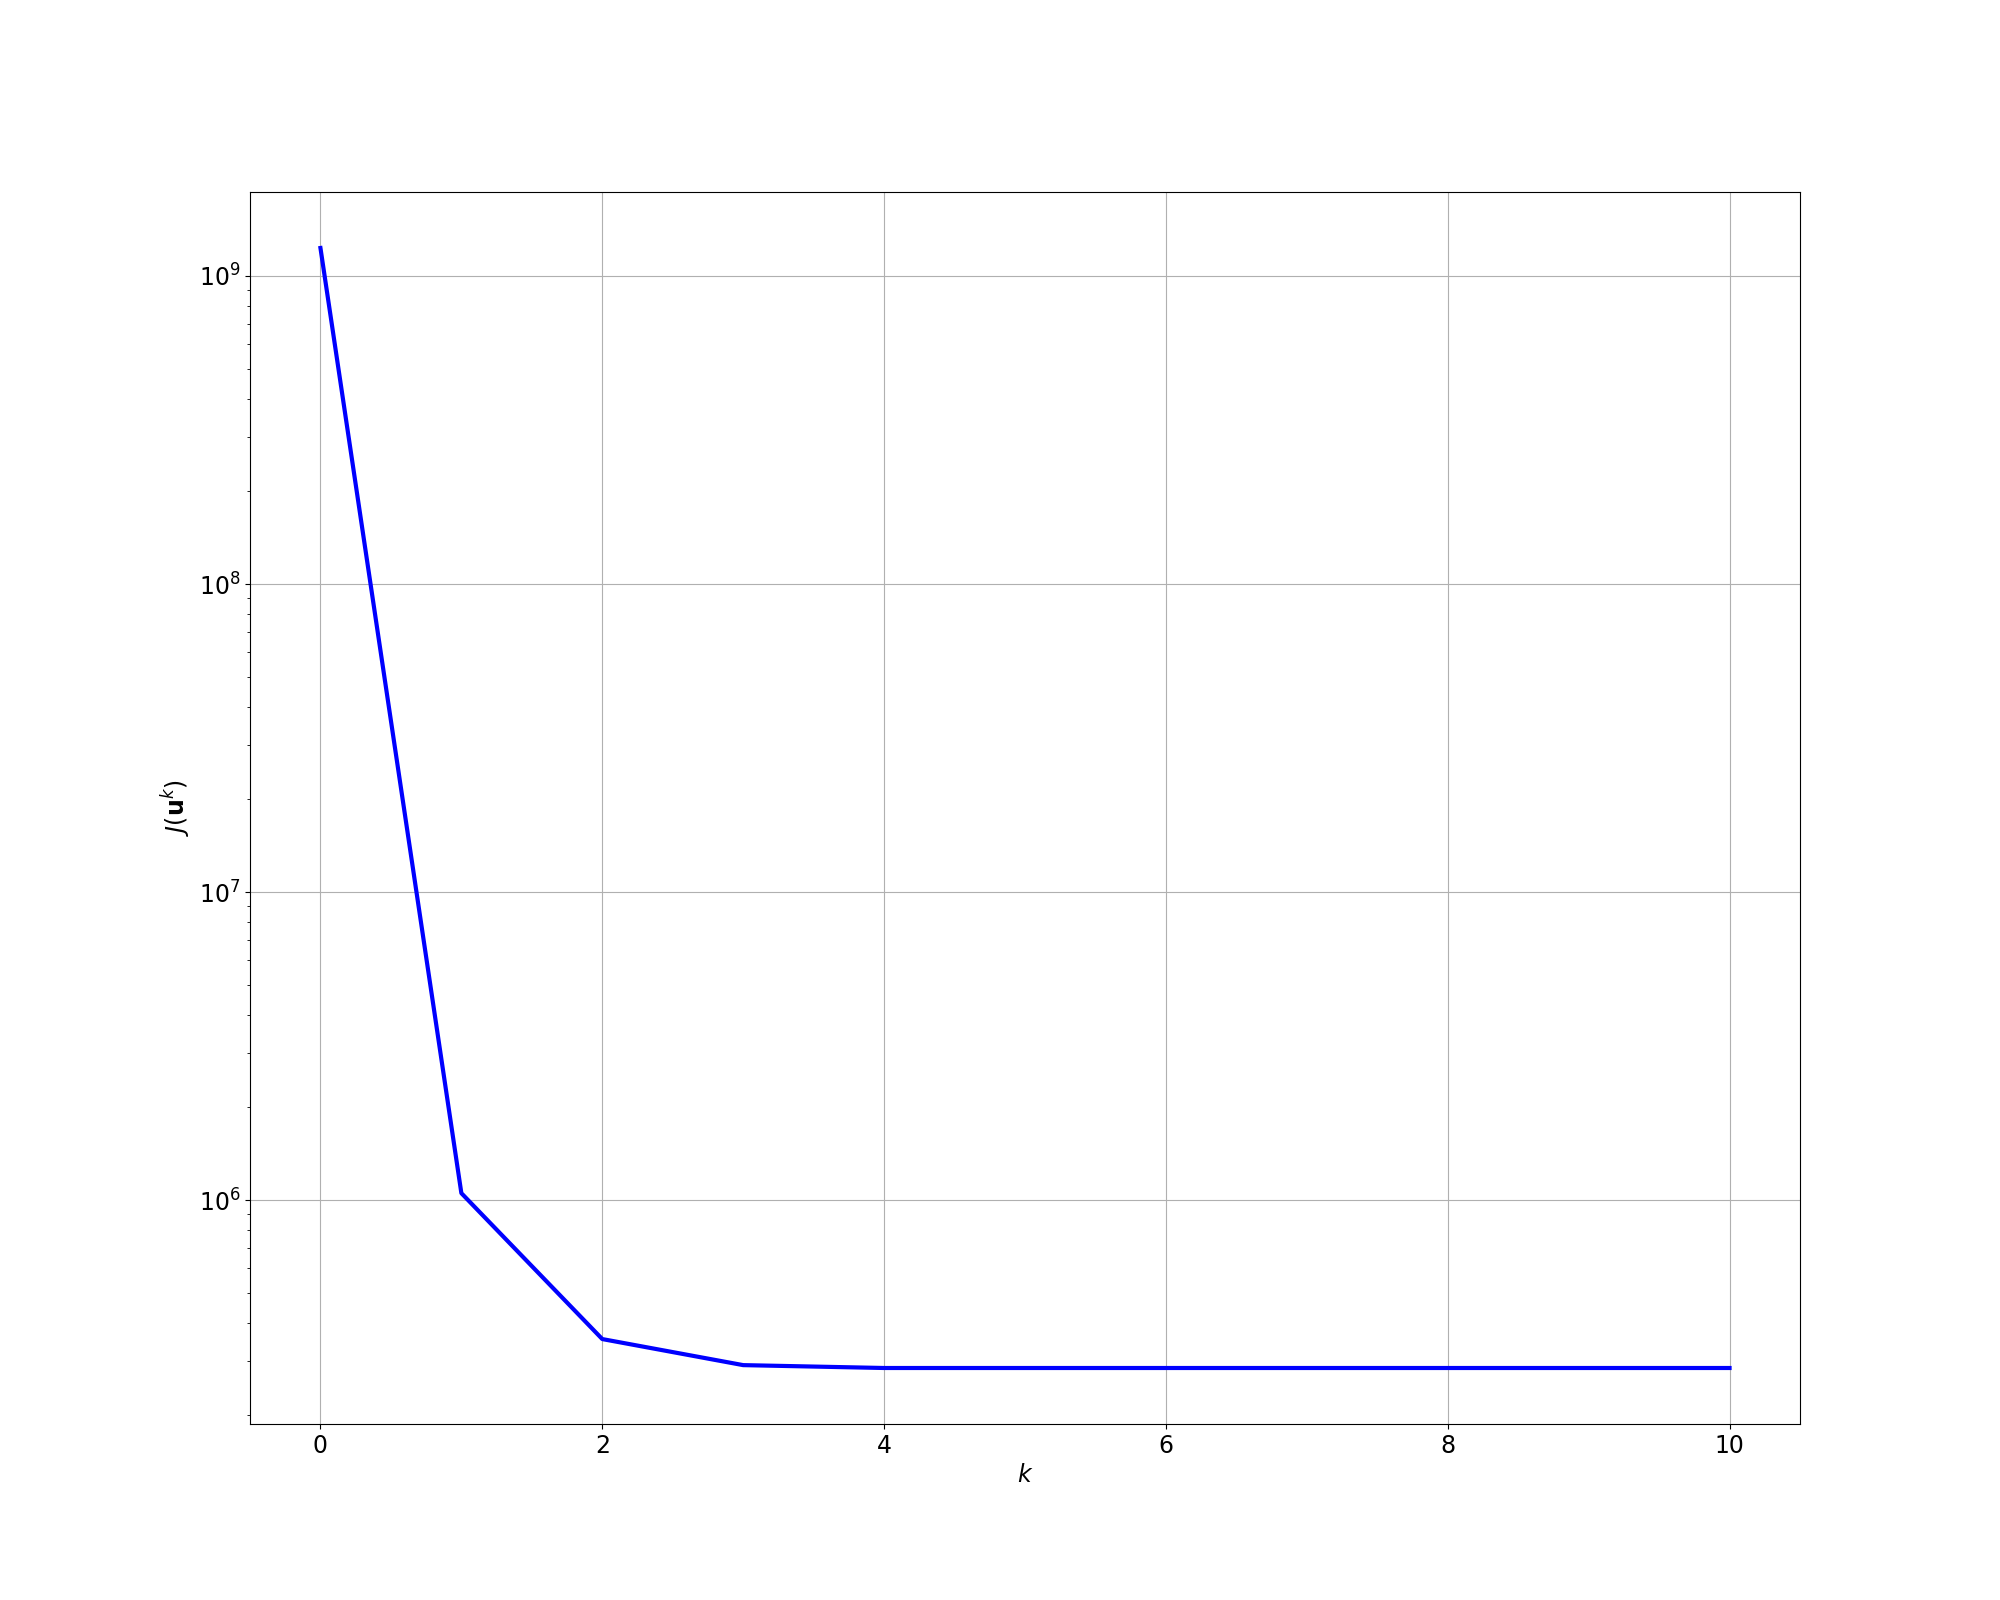
\includegraphics[scale=.2]{figs/Task2/cost} \\
    \caption{Cost's plot}
    \label{fig:enter-label}
\end{figure}

\begin{figure}[h]
    \centering
    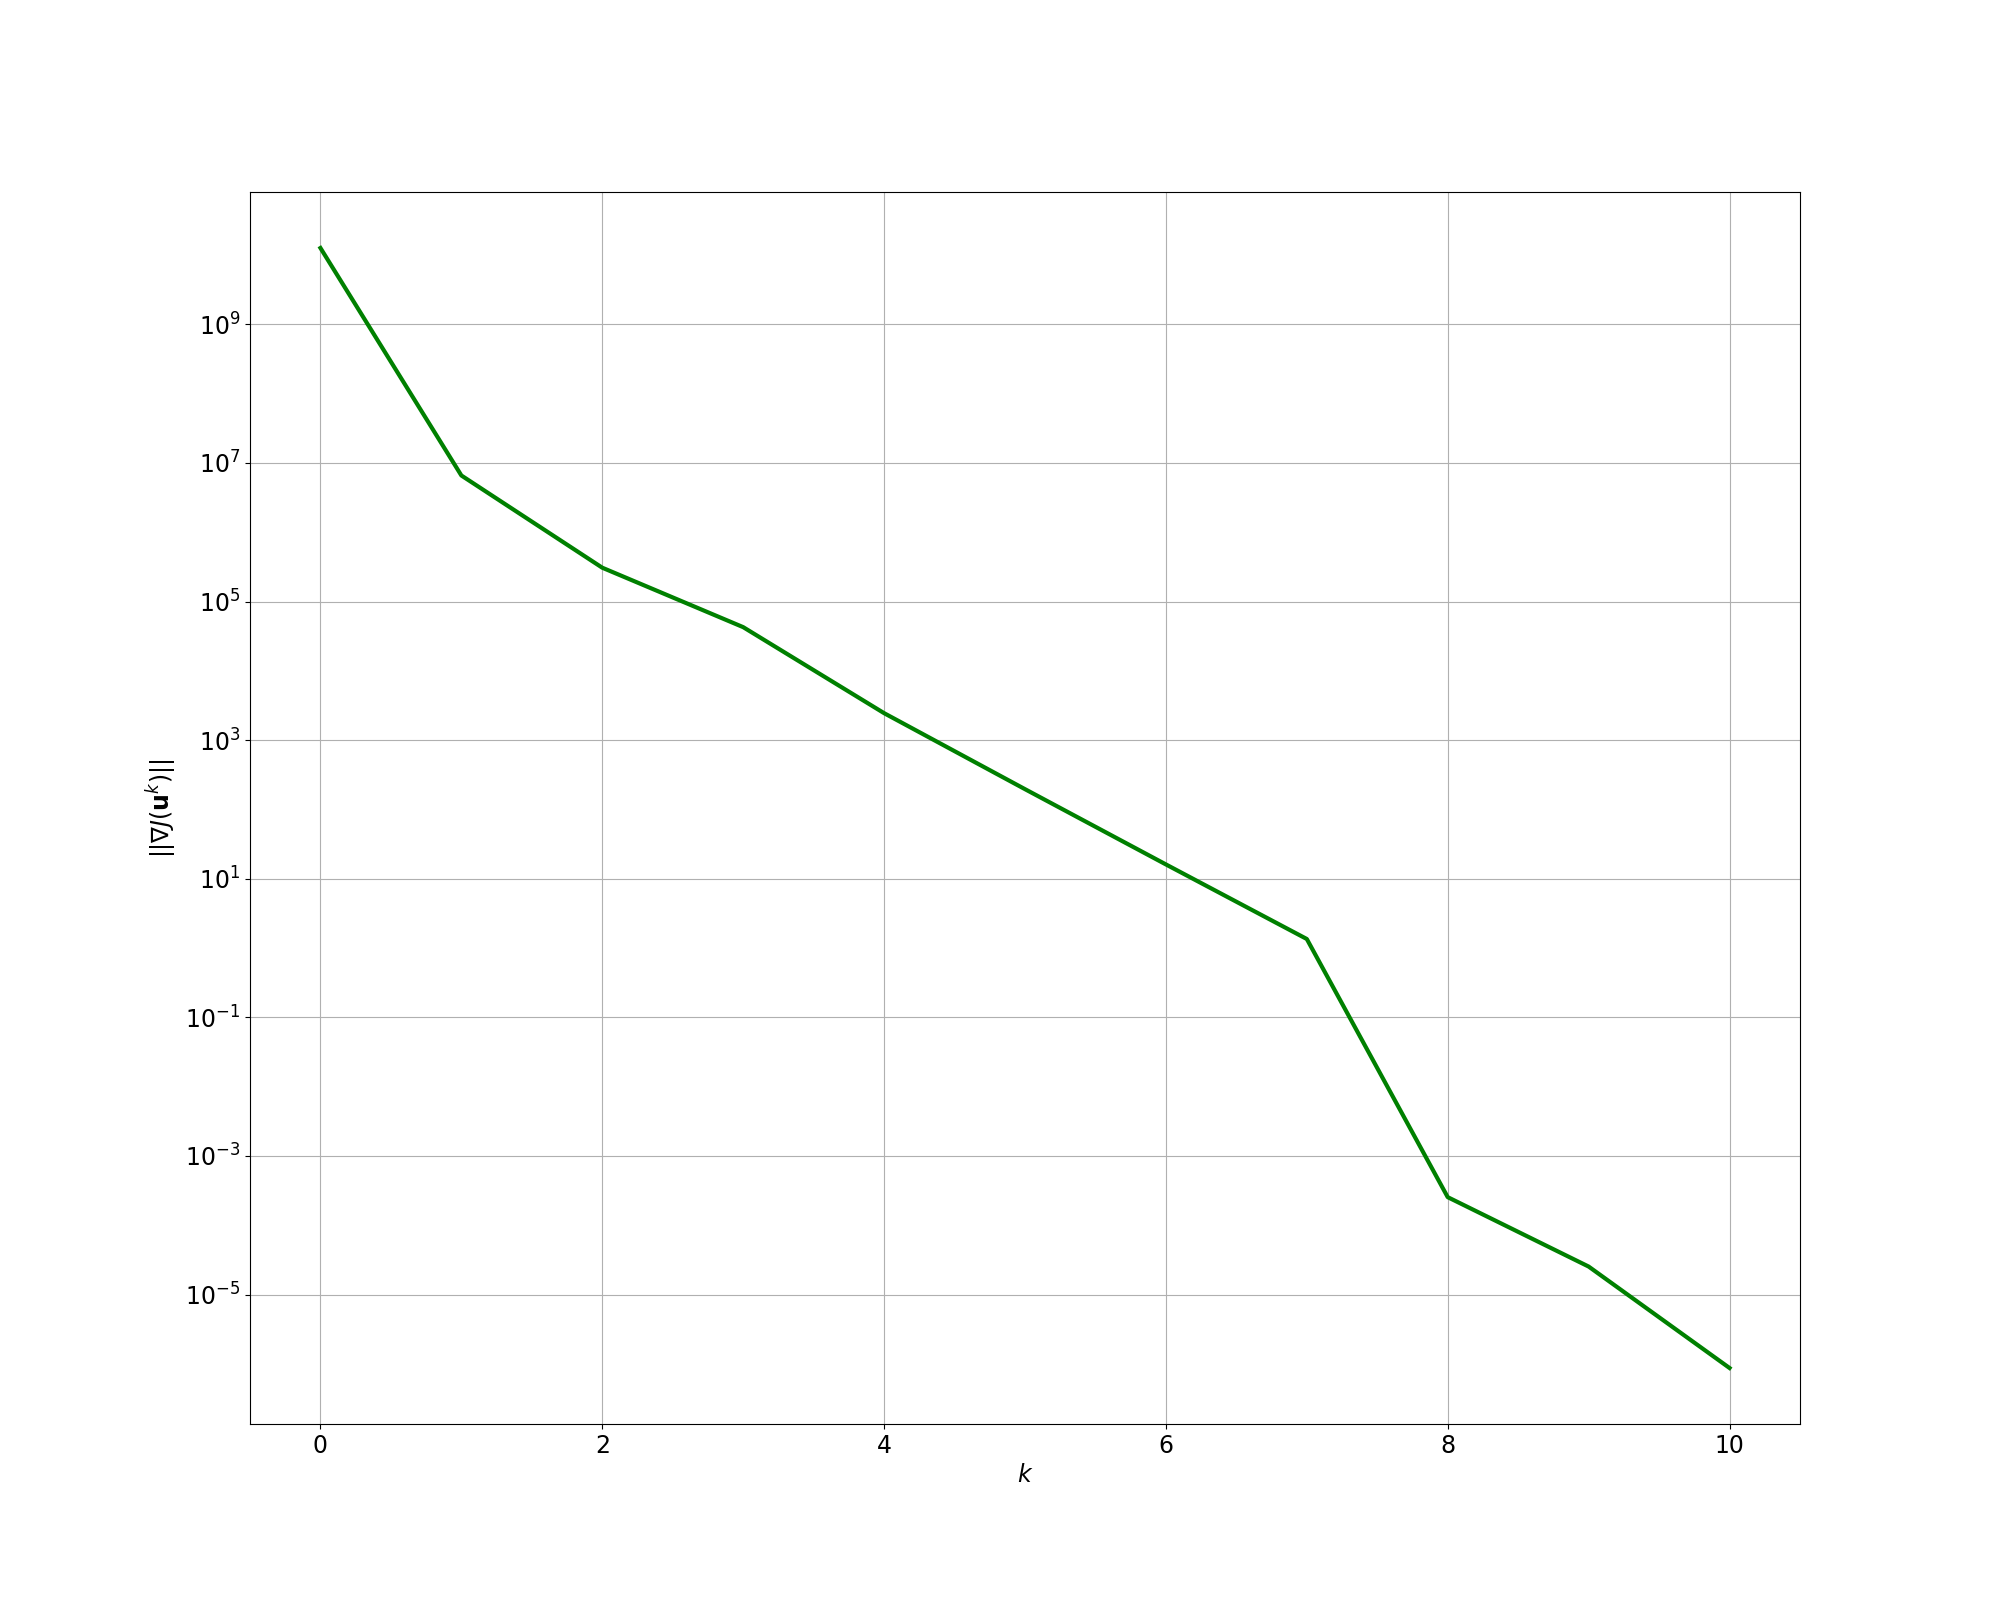
\includegraphics[scale=.2]{figs/Task2/descent_direction} \\
    \caption{Descent direction's plot}
    \label{fig:enter-label}
\end{figure}
\newpage
\subsection{Sub-optimal trajectories}
The following first plot shows the optimal trajectory found at iterations 0, 2, and 10. From this image, it is possible to observe the improvement of the trajectory as the iterations progress.\\

The other ones shows for iterations 0, 2, and 10:
\begin{itemize}
    \item Optimal trajectory including all states and inputs
    \item Armijo's plot
\end{itemize}
\begin{figure}[h]
    \centering
    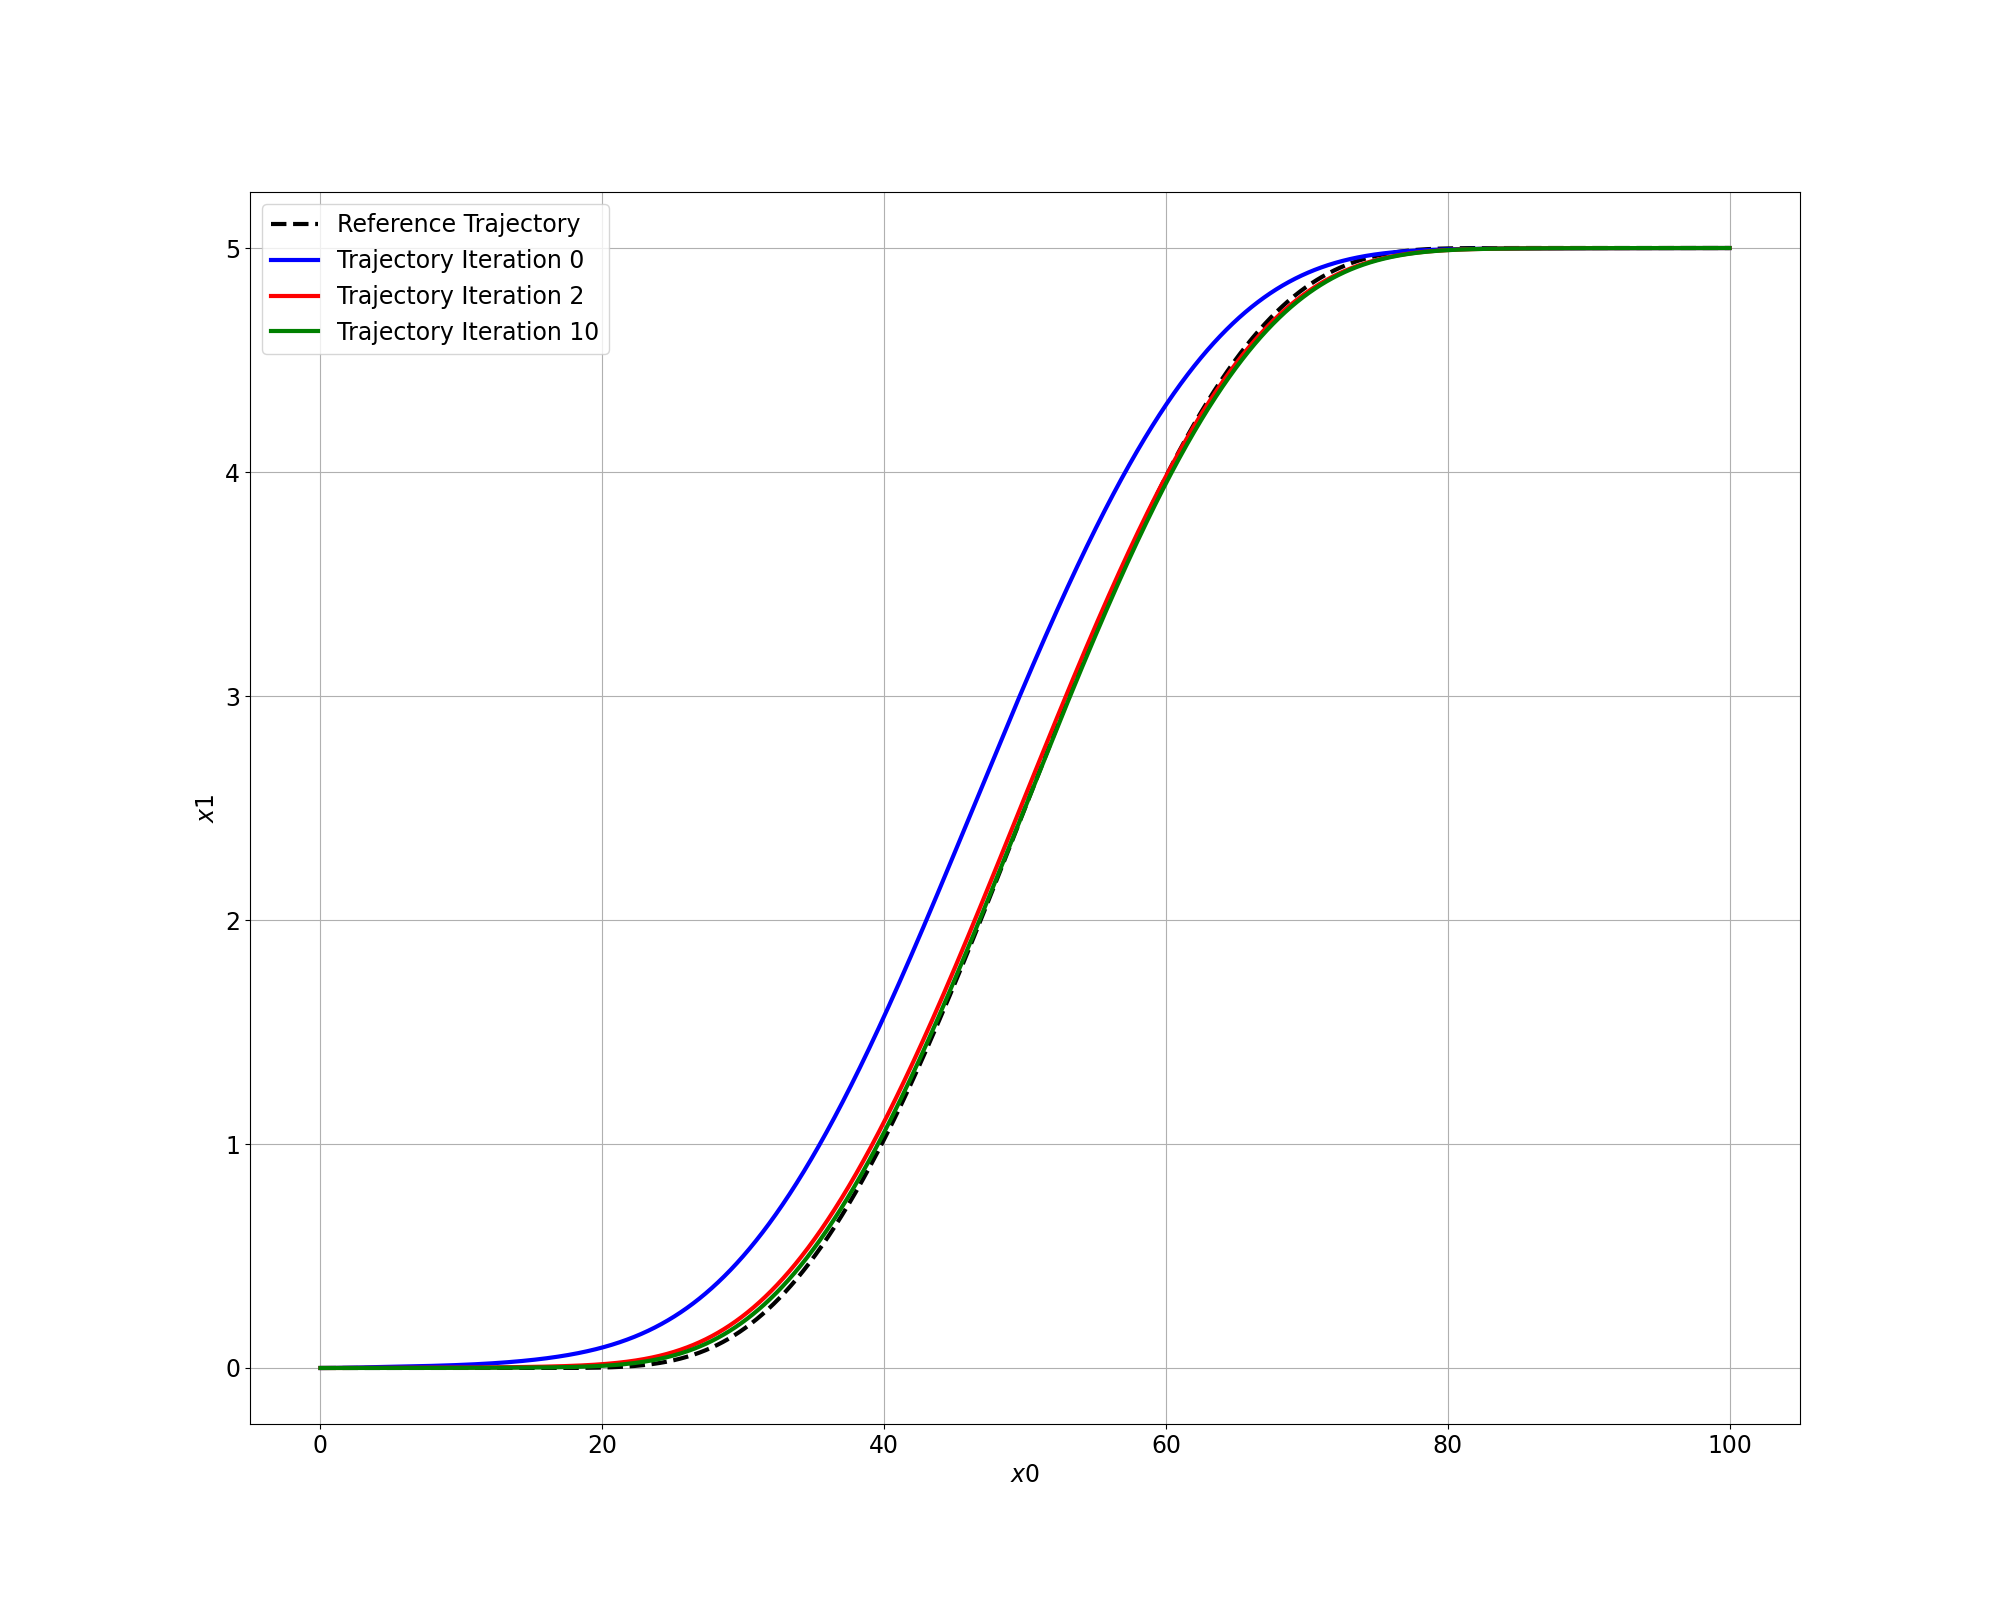
\includegraphics[scale=.3]{Report_OPTCON_Project/figs/Task2/XYintermediate.png} \\
    \caption{Sub-optimal trajectory for iteration 0,2 and 10}
    \label{fig:sub-opt}
\end{figure}

\begin{figure}[t]
    \centering
    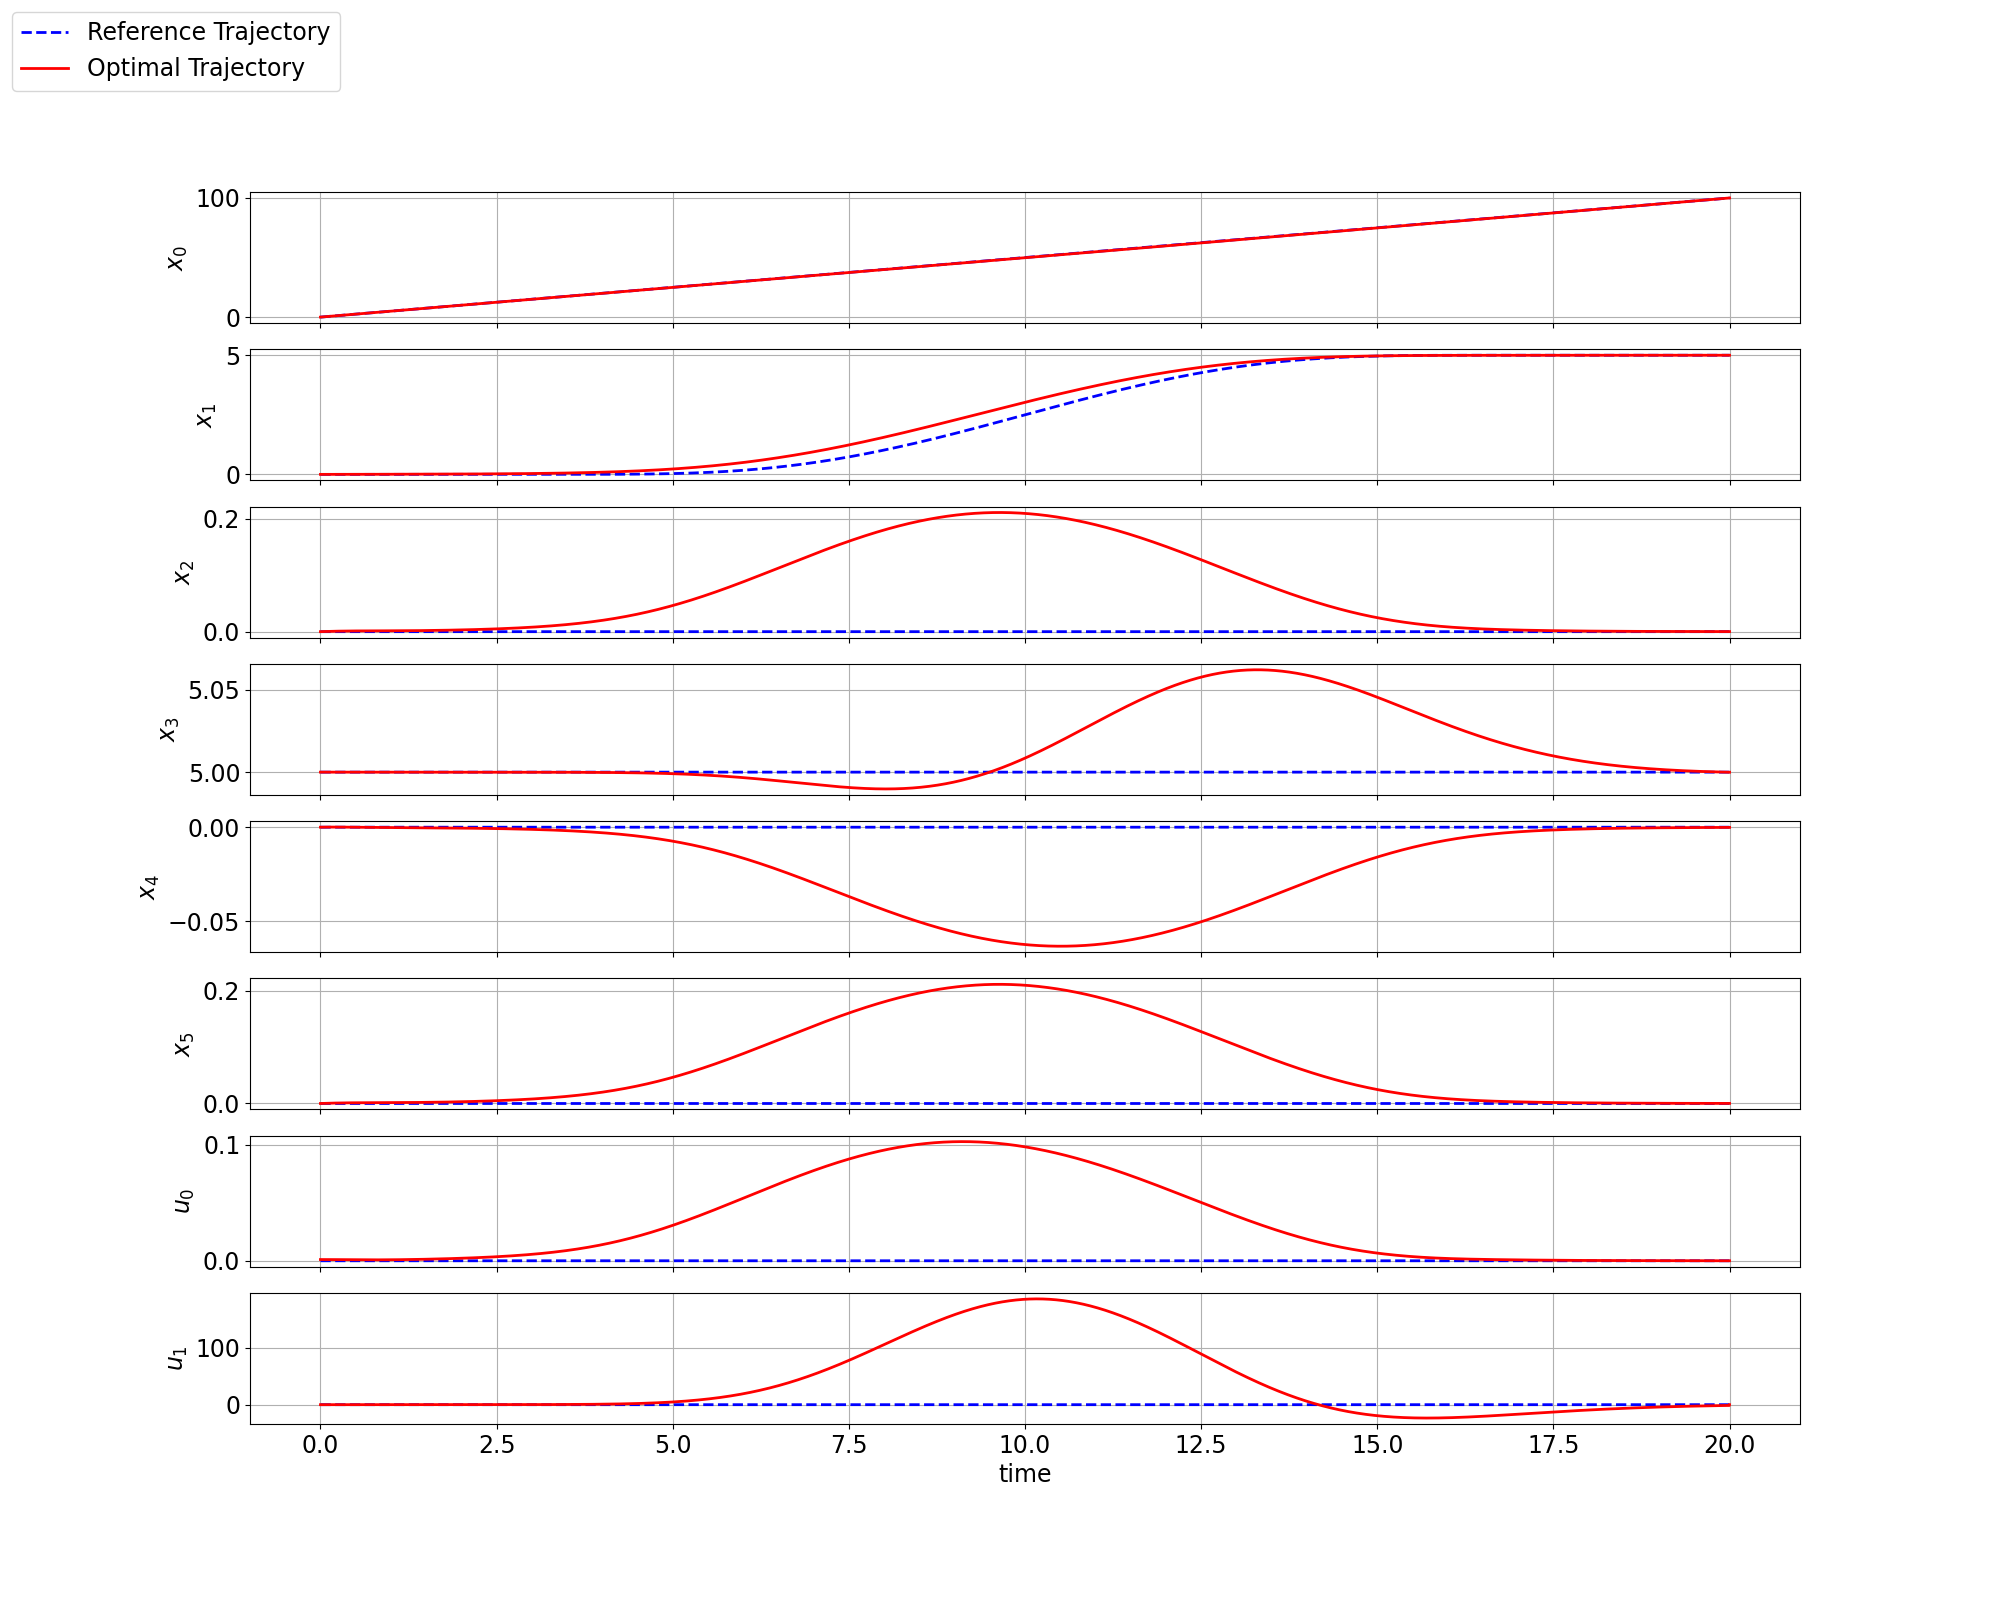
\includegraphics[scale=.25]{Report_OPTCON_Project/figs/Task2/opt_traj_iter0.png} \\
    \caption{Optimal trajectory iteration 0}
    \label{fig:optimal0}
\end{figure}
\begin{figure}[h]
    \centering
    \includegraphics[scale=.25]{Report_OPTCON_Project/figs/Task2/armijo_plot_0.png} \\
    \caption{Armijo's plot iteration 0}
    \label{fig:armijo0}
\end{figure}

\begin{figure}[t]
    \centering
    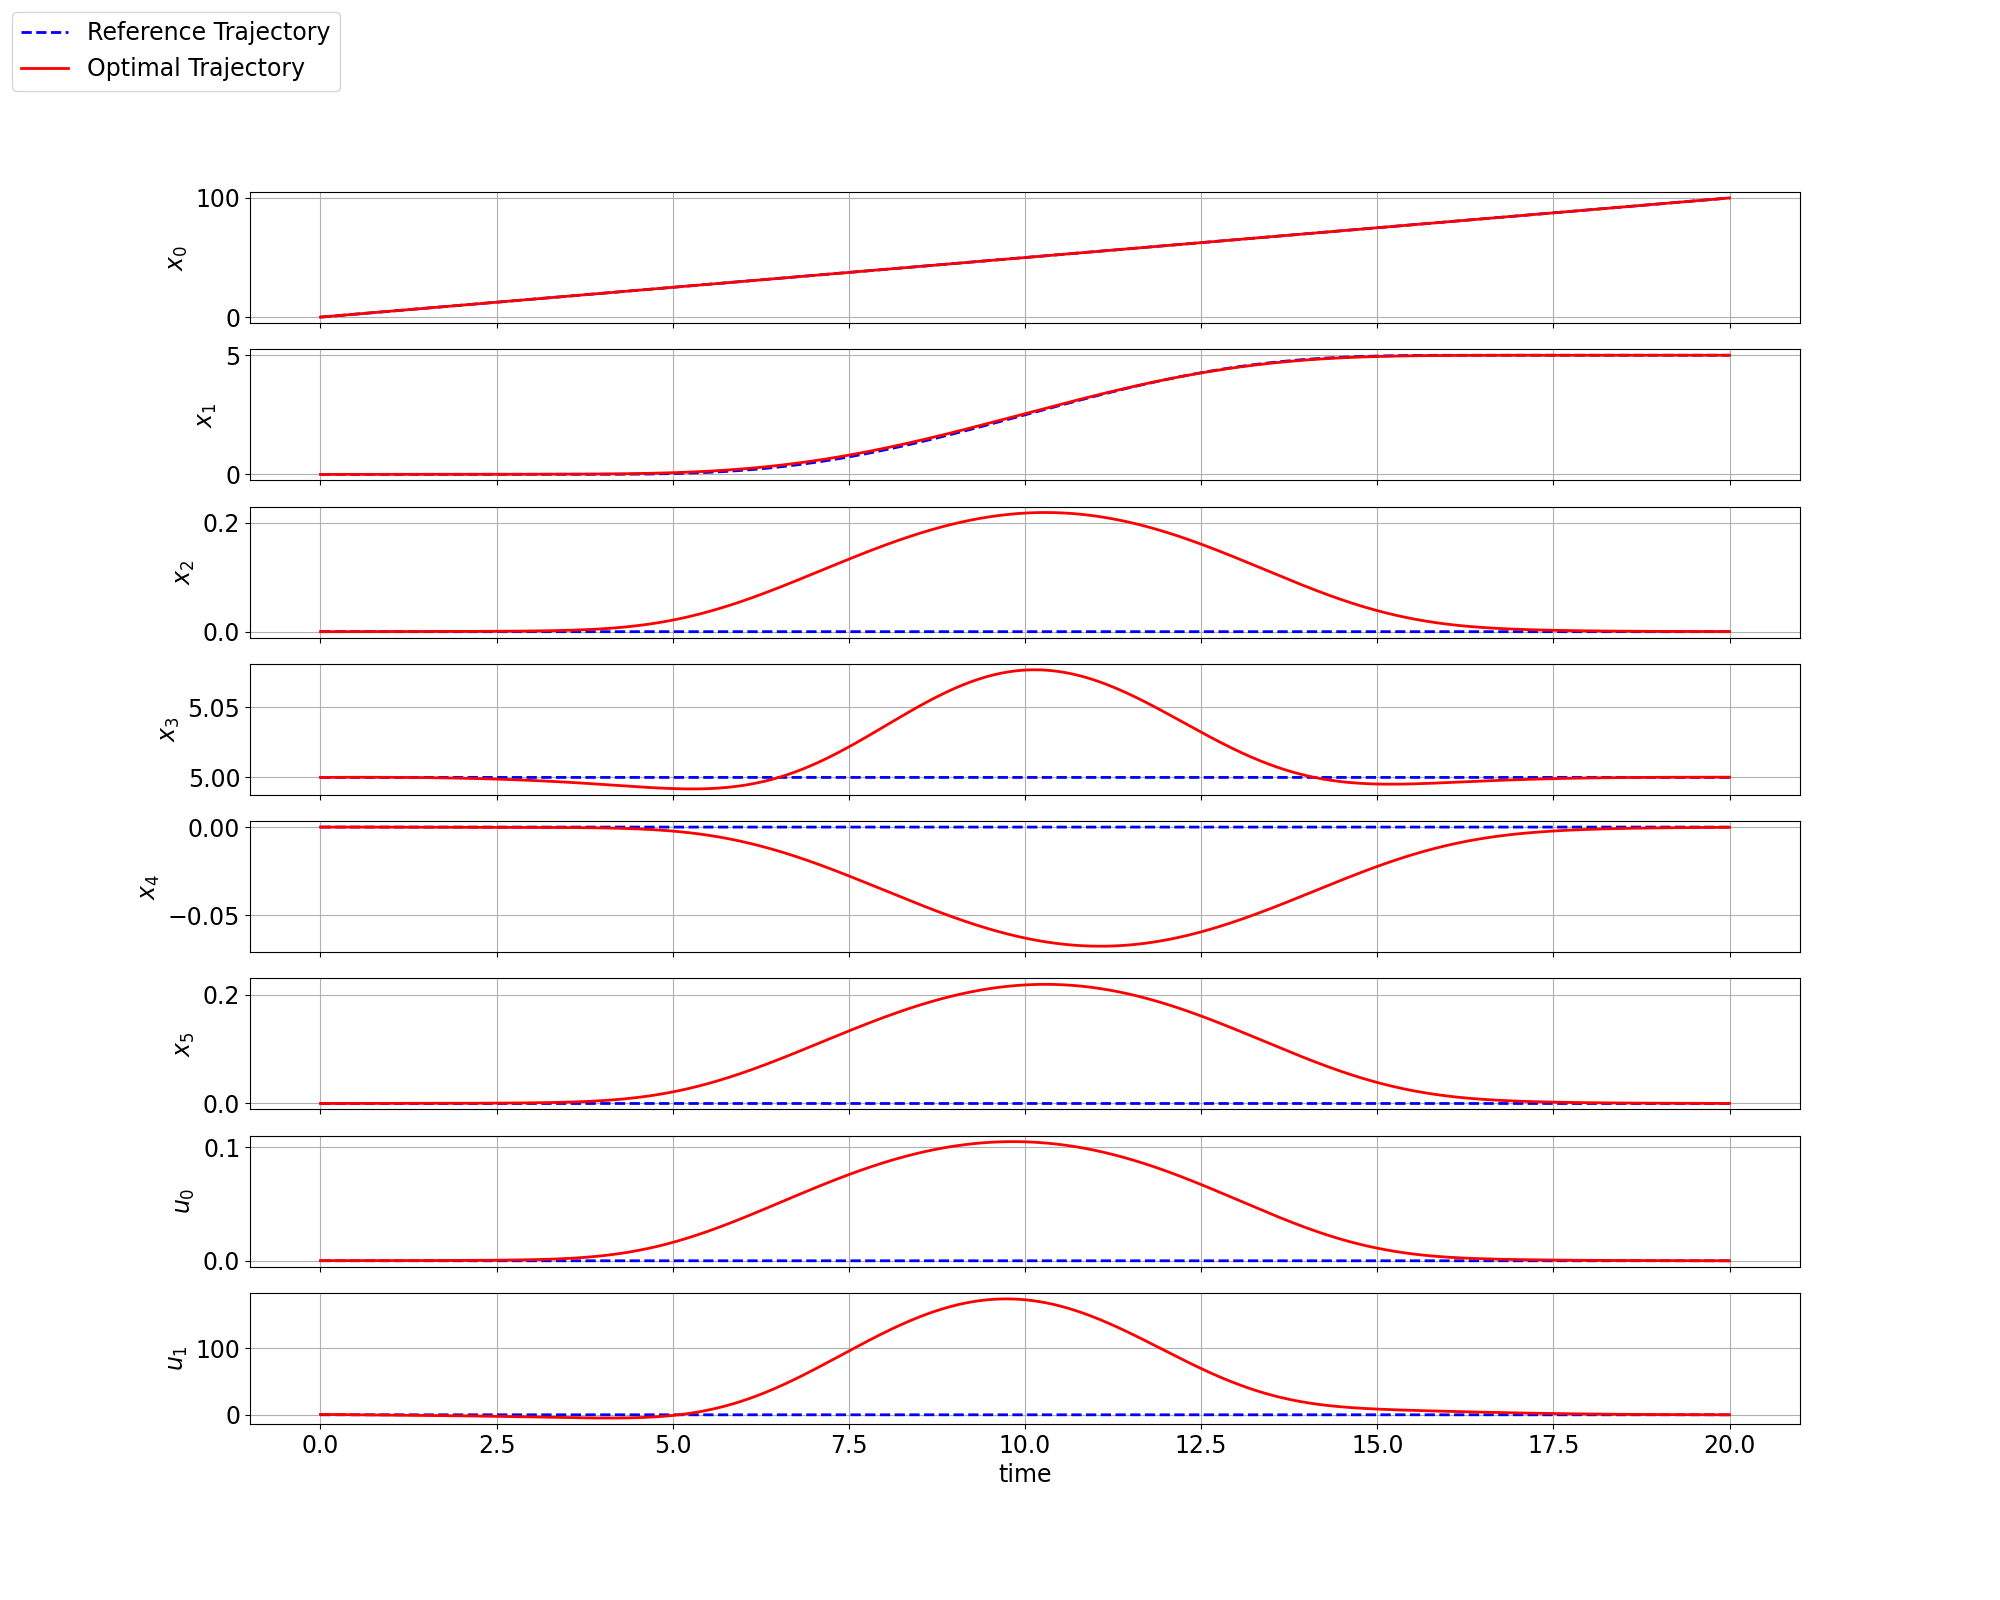
\includegraphics[scale=.25]{Report_OPTCON_Project/figs/Task2/opt_traj_iter2.png} \\
    \caption{Optimal trajectory iteration 2}
    \label{fig:optimal2}
\end{figure}
\begin{figure}[h]
    \centering
    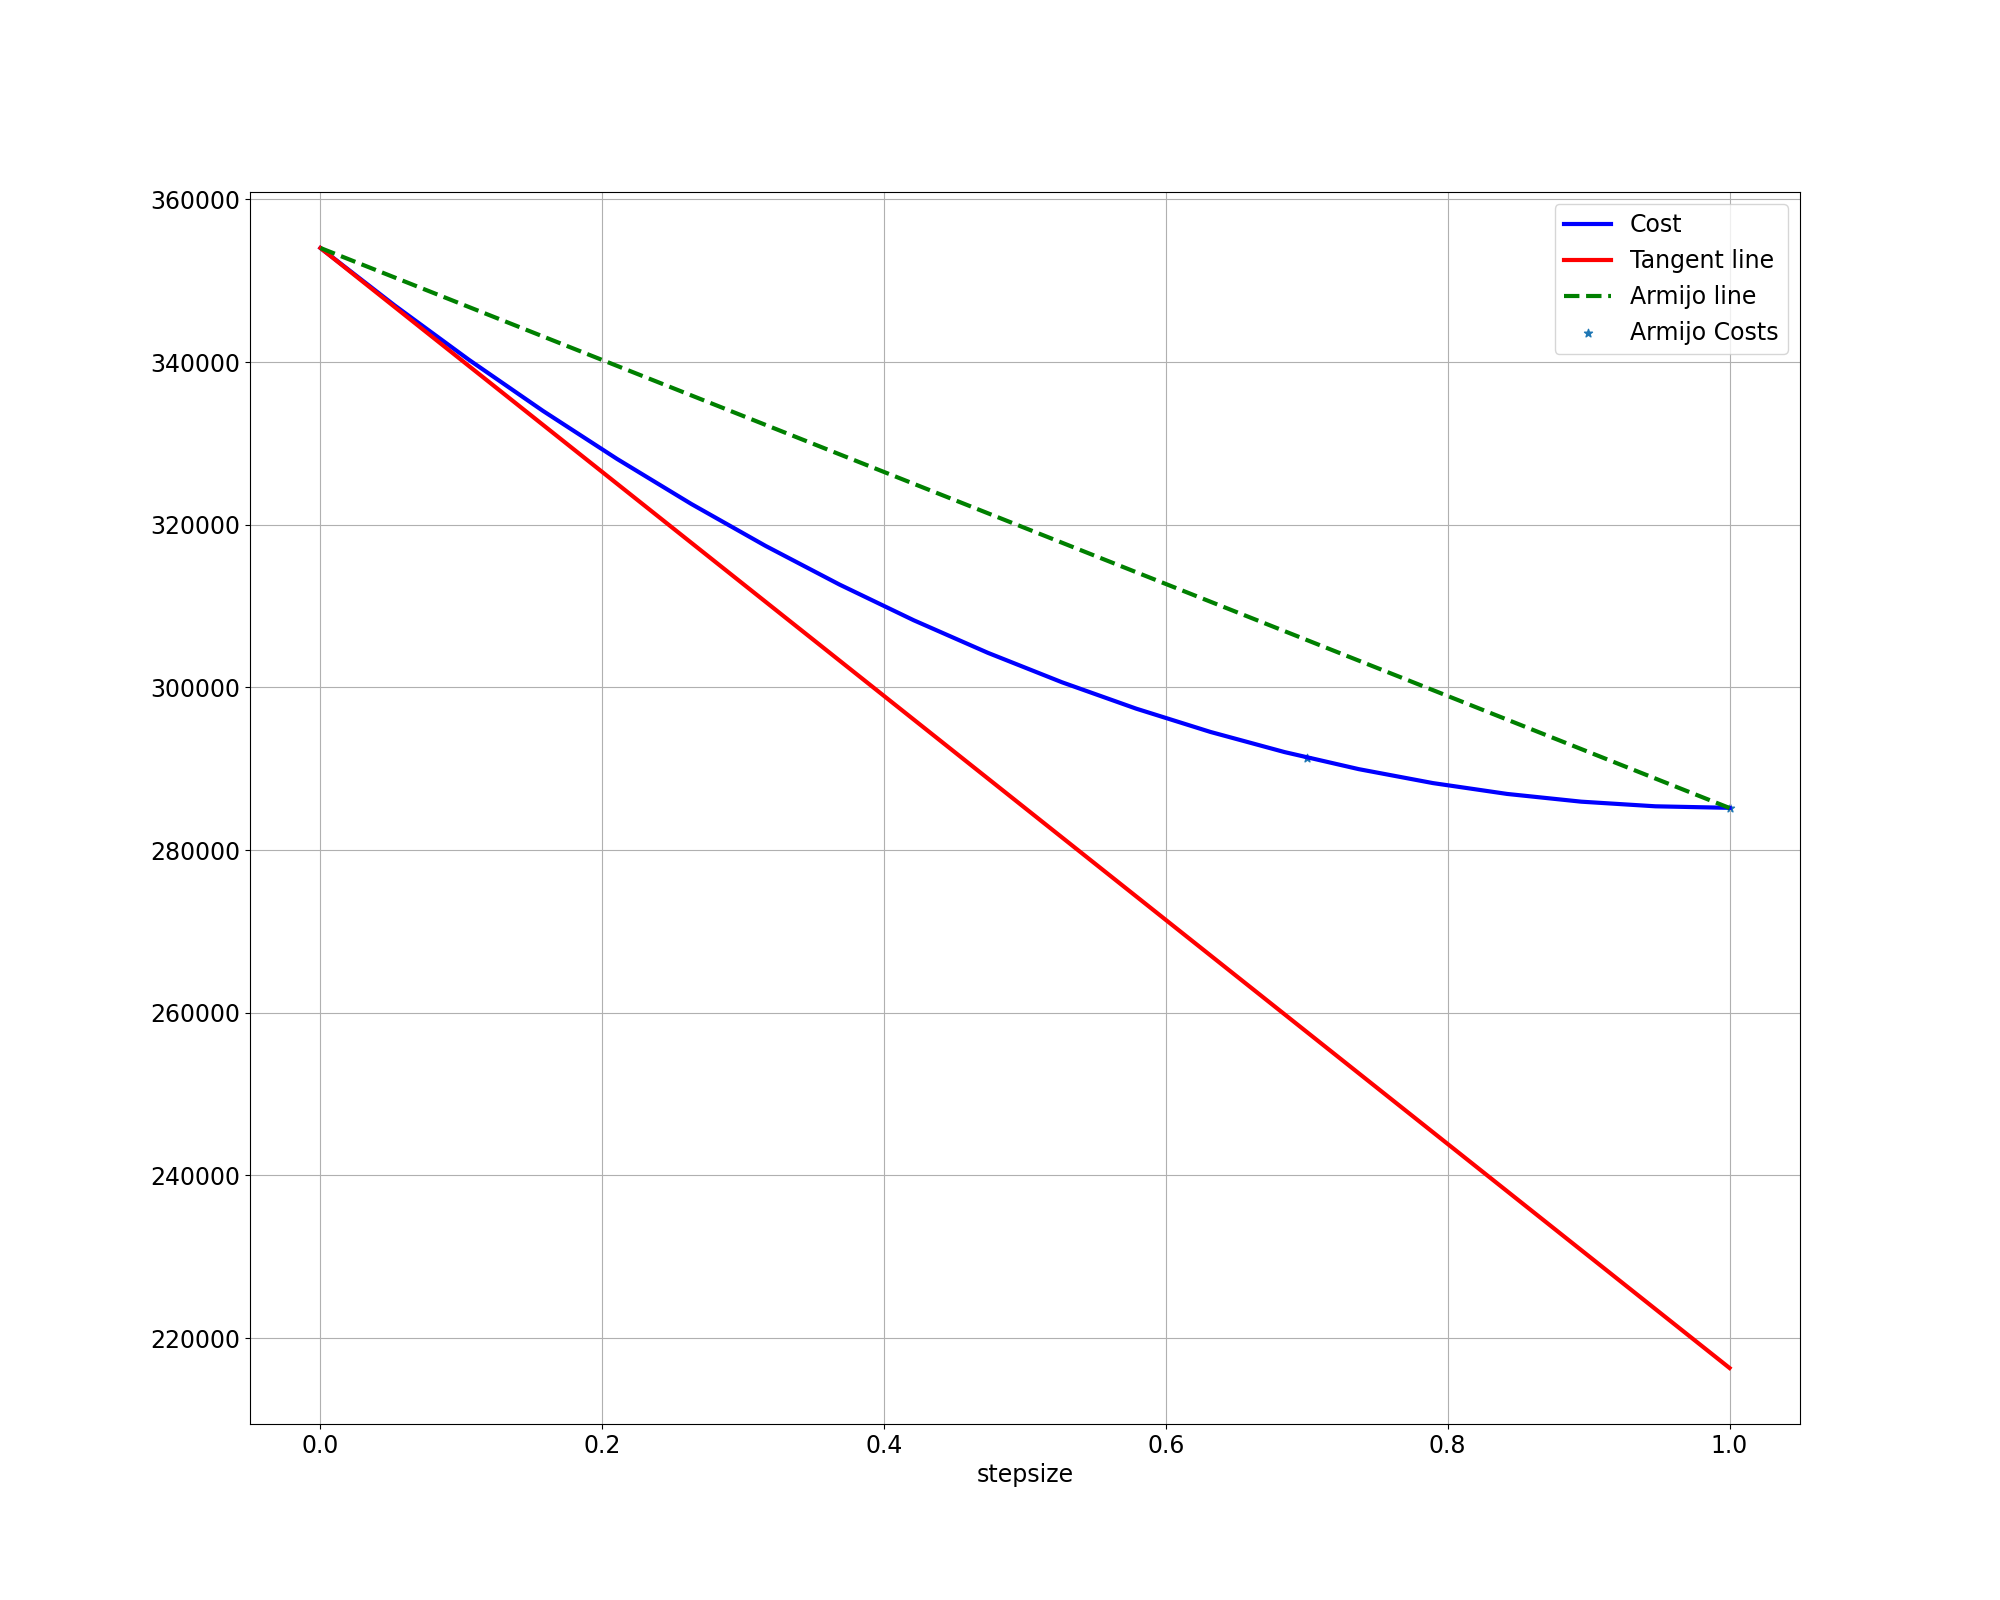
\includegraphics[scale=.25]{Report_OPTCON_Project/figs/Task2/armijo_plot_2.png} \\
    \caption{Armijo's plot iteration 2}
    \label{fig:armijo2}
\end{figure}

\begin{figure}[t]
    \centering
    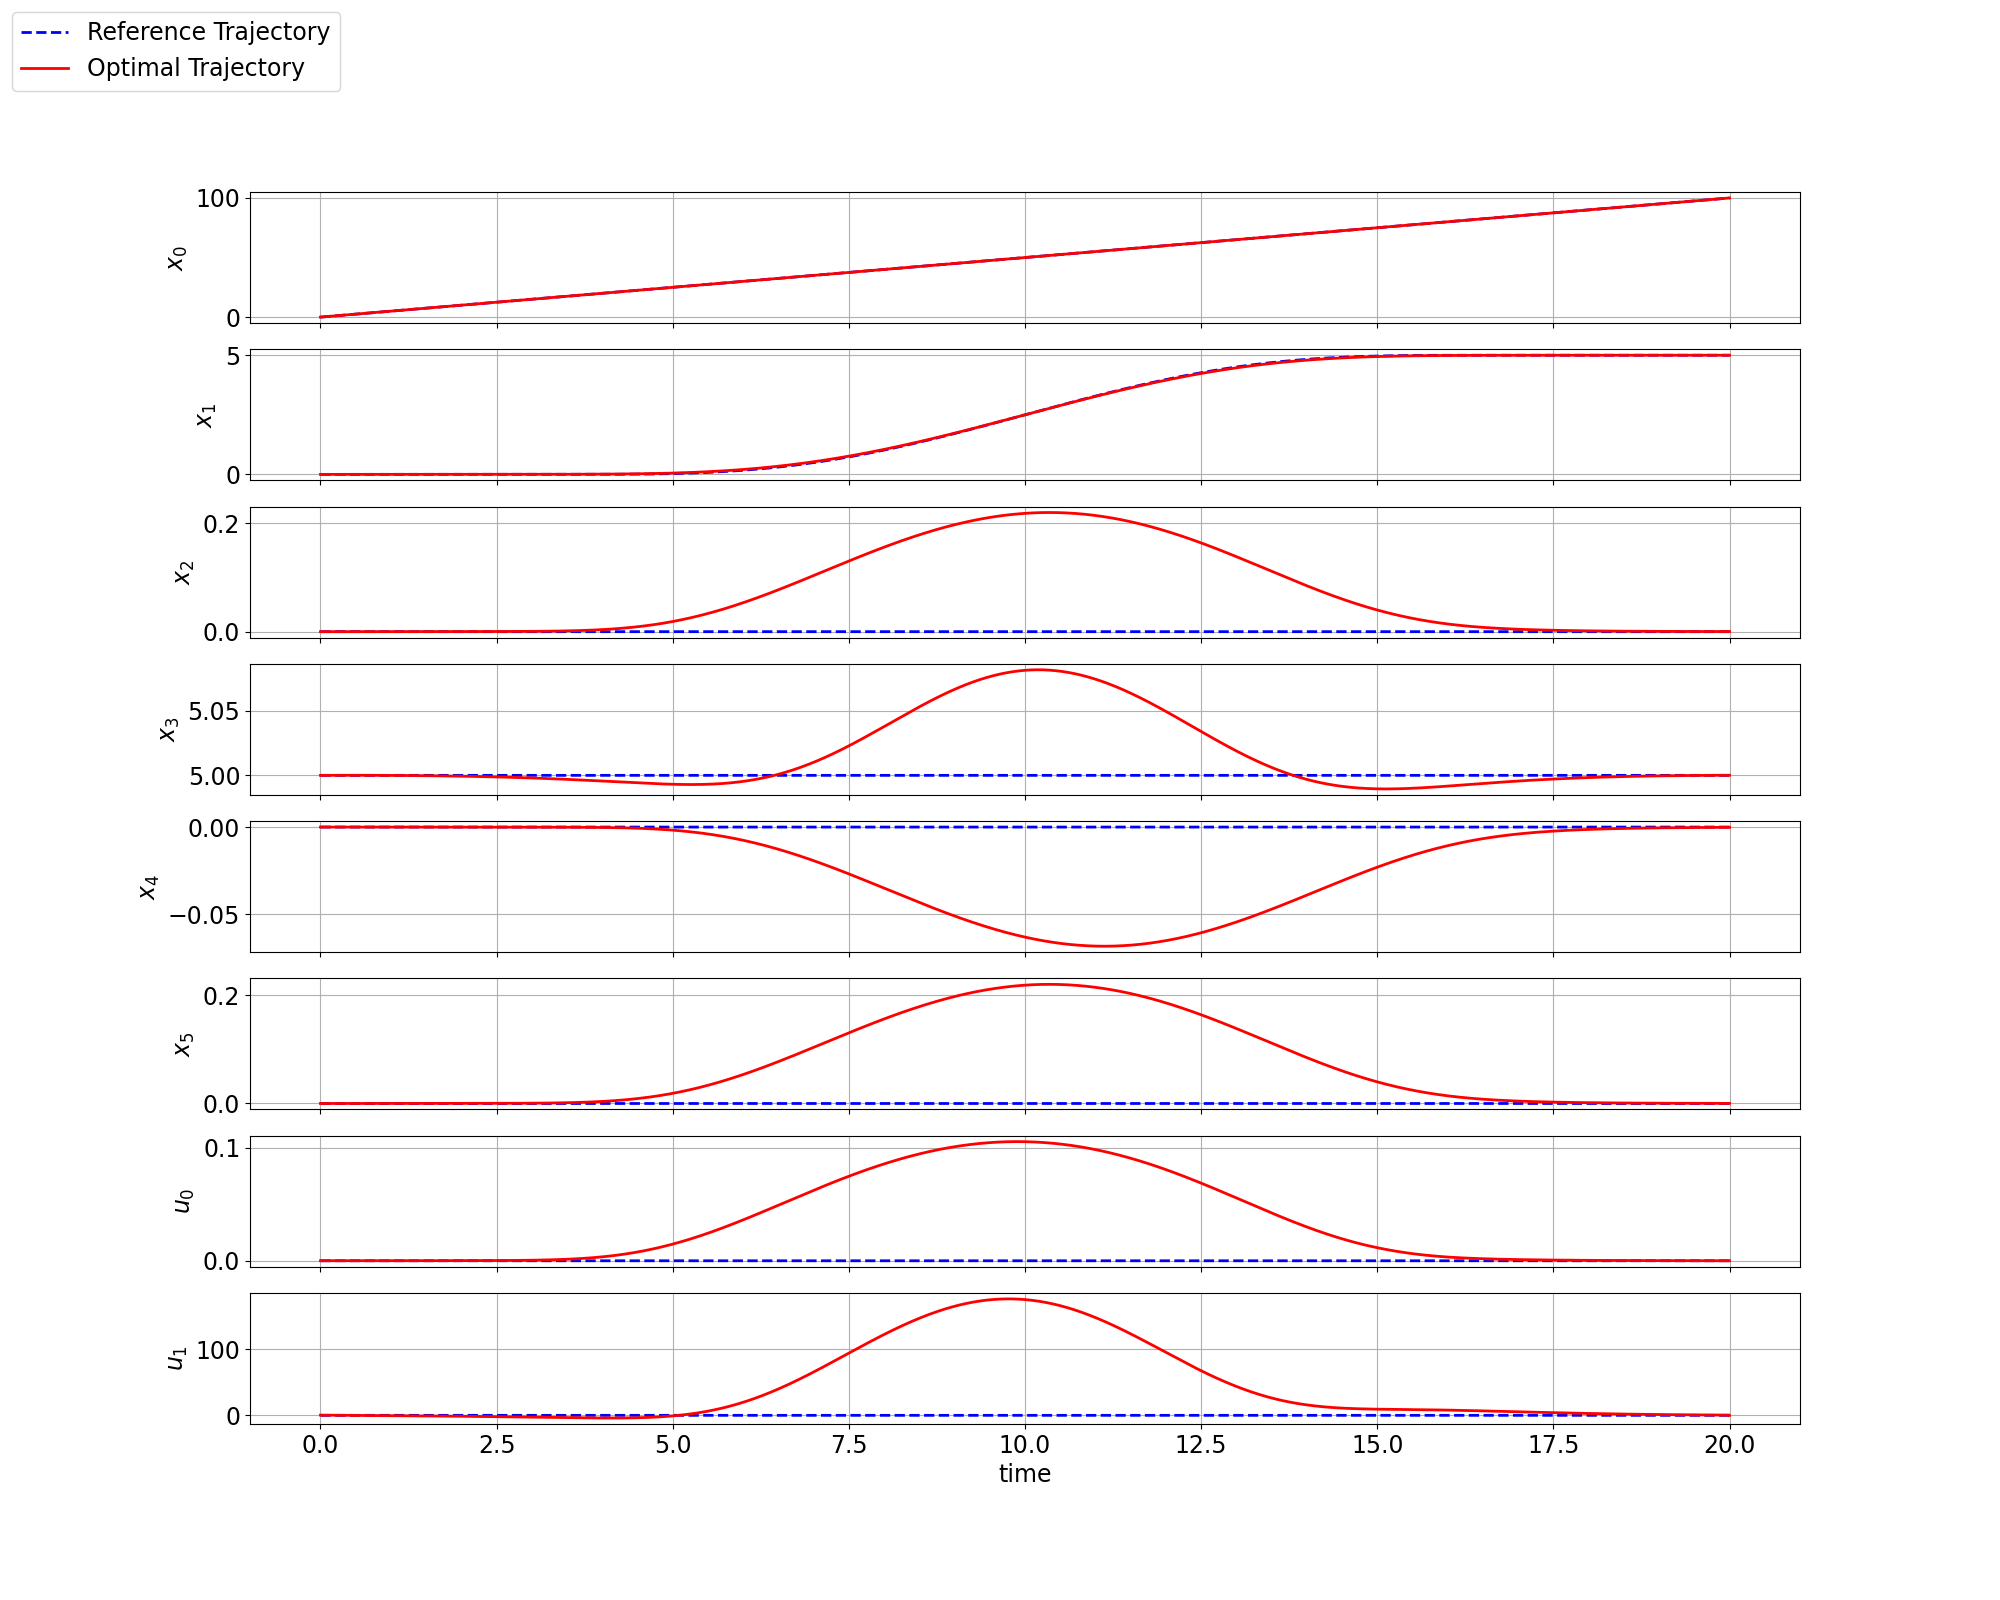
\includegraphics[scale=.25]{Report_OPTCON_Project/figs/Task2/opt_traj_iter10.png} \\
    \caption{Optimal trajectory iteration 10}
    \label{fig:optimal10}
\end{figure}
\begin{figure}[h]
    \centering
    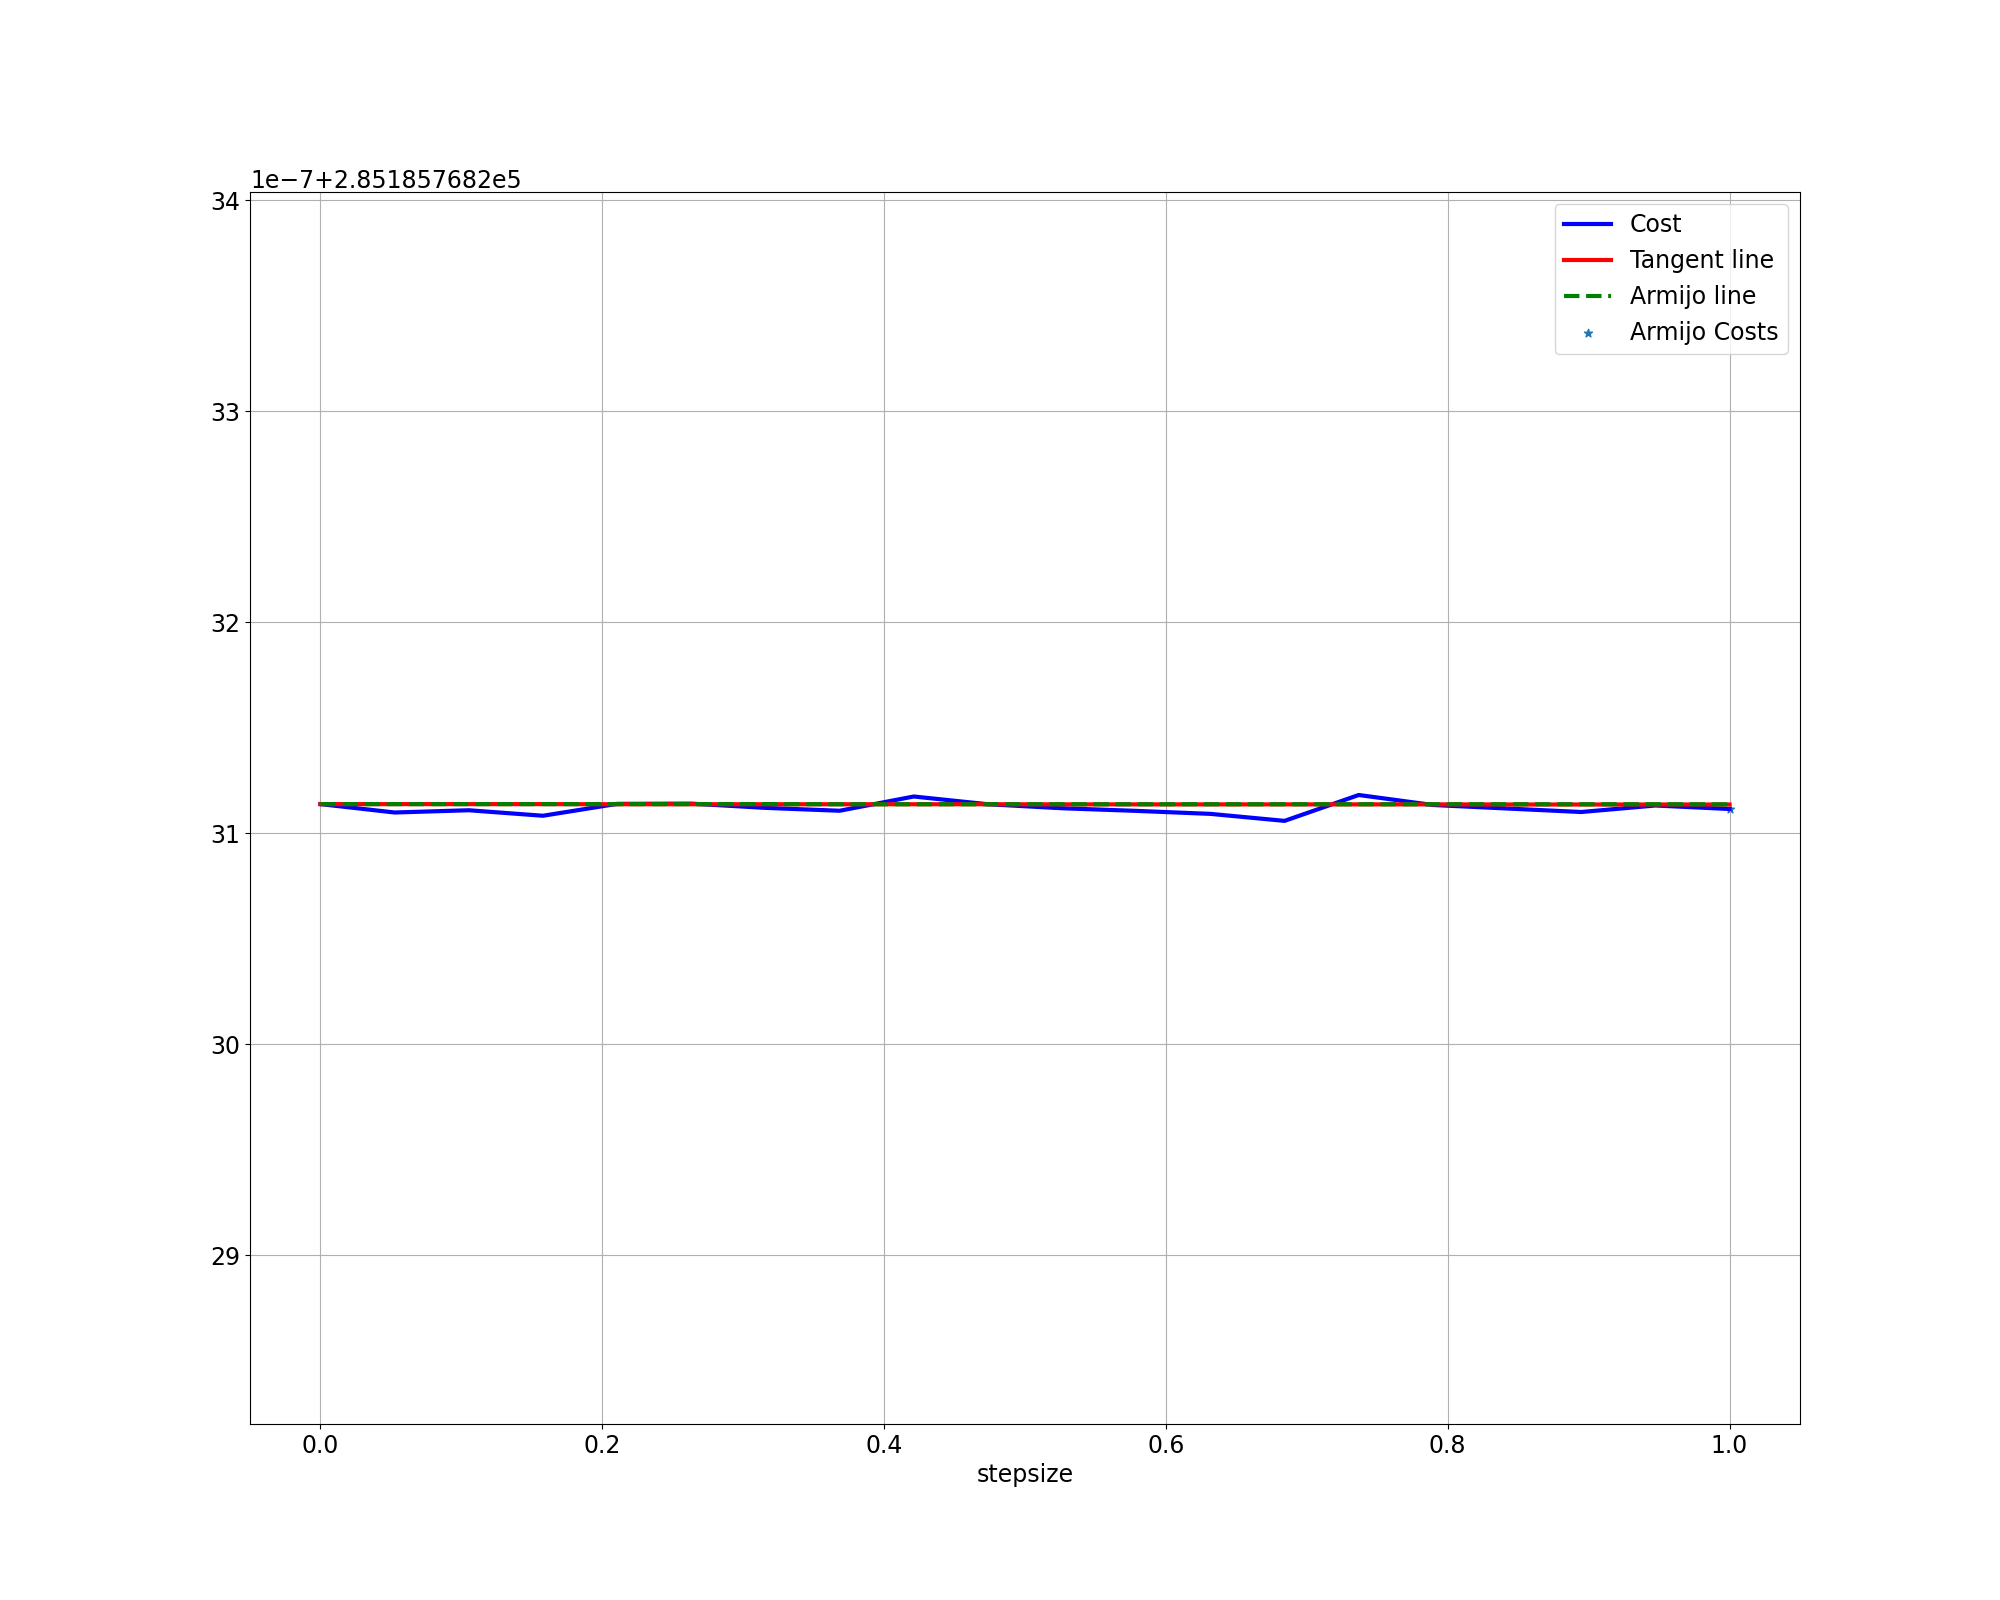
\includegraphics[scale=.25]{Report_OPTCON_Project/figs/Task2/armijo_plot_10.png} \\
    \caption{Armijo's plot iteration 10}
    \label{fig:armijo10}
\end{figure}

%%%%%%%%%% Task 3 %%%%%%%%%%
\chapter{Task 3 - Trajectory tracking via LQR} \label{chapter:task3}
Linearizing the vehicle dynamics about the (optimal) trajectory $(x^{opt}, u^{opt})$ computed in Task 2 (chapter \ref{chapter:task2}), exploit the LQR algorithm to define the optimal feedback controller to track this reference trajectory.\\
In particular, you need to solve the LQ Problem\\
\[
\min_{\substack{\Delta x_1, \cdots, \Delta x_T};\\ 
\atop \Delta u_o, \cdots, \Delta u_{T-1}}}
\sum_{t=0}^{T-1} \Delta x_t^T Q^{reg} \Delta x_t + \Delta u_t^T R^{reg} \Delta u_t + \Delta x_T^T Q_T^{reg} \Delta x_T\\
\]
\\
\[
\text{subj.to }\Delta x_{t+1} = A_t^{opt} \Delta x_t + B_t^{opt} \Delta u_t \ \ \ \  t=0,...,T-1 \\
\]
\[
x_0 = 0 
\]
\section{LQR-based trajectory tracking}
The idea is to track the generated (optimal) trajectory $(x^{opt},u^{opt})$ via a (stabilizing)  feedback Linear Quadratic Regulator (LQR) on the linearization.\\
Applying the feedback controller designed on the linearization to the nonlinear system, it's possible to track $(x_t,u_t)$.\\
Namely, for all $t=0,...,T-1$ [$T-1$ is finite horizon] it applies
\begin{align*}
    u_t = u_t^{opt} &+ K_t^{reg} (x_t-x_t^{opt})\\
    x_{t+1} &= f_t(x_t,u_t)
\end{align*}
\begin{center}
    with x0 given.\\
\end{center}
The nominal trajectory and the feedback gains have been computed on a finite horizon of length T.
\section{Costs definition}
The cost matrices employed in this task are the same as those used in Task 2 (chapter \ref{chapter:task2}). This decision stems from the constancy in significance attributed to the state and input elements, which has persisted unchanged.
\begin{center}
    $Q_t$ = \begin{bmatrix}
                100 & 0 & 0 & 0 & 0 & 0\\
                0 & 1000 & 0 & 0 & 0 & 0\\
                0 & 0 & 10 & 0 & 0 & 0\\
                0 & 0 & 0 & 100 & 0 & 0\\
                0 & 0 & 0 & 0 & 100 & 0\\
                0 & 0 & 0 & 0 & 0 & 10\\
            \end{bmatrix}
    $R_t$ = \begin{bmatrix}
                10000 & 0\\
                0 & 0.0001\\
            \end{bmatrix}
\end{center}
\begin{center}
$Q_T$ = solution of Riccati equation
\end{center}

\section{Results}
In Figure \ref{fig:opt_traj_task3} can be observed the plot of the trajectory tracked via LQR in relation to the desired optimal trajectory for all states and inputs.\\
To assess how well the controller tracks the desired trajectory, the vehicle's starting position is intentionally varied from the optimal trajectory. The plot in Figure \ref{fig:opt_traj_task3} illustrate instances of the controller's tracking performance.\\
\begin{figure}[h]
    \centering
    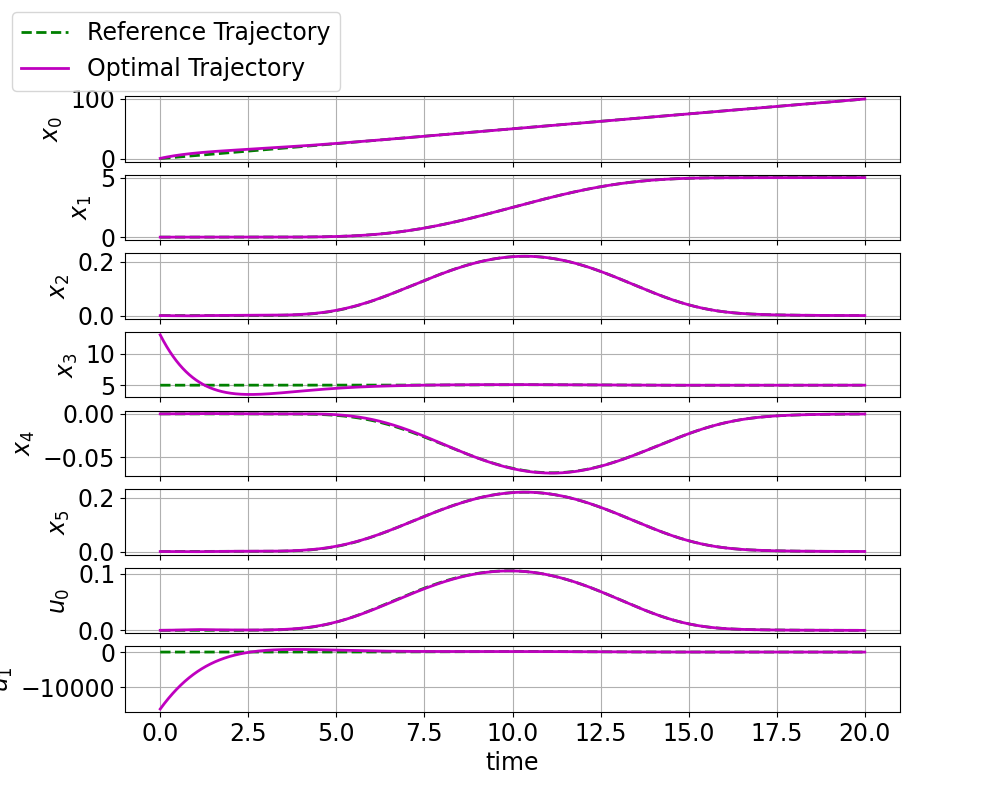
\includegraphics[scale=.50]{Report_OPTCON_Project/figs/Task3/TASK3_opt_trajectory.png} \\
    \caption{Optimal trajectory}
    \label{fig:opt_traj_task3}
\end{figure}
\newpage
Given the perturbed inputs as follows: 
\begin{center}
    $x_0=[-30, 0, 0, 8, 0, 0]^T$
\end{center}
The plot in Figure \ref{fig:error_task3} shows the tracking error for different initial conditions.
\begin{figure}[h]
    \centering
    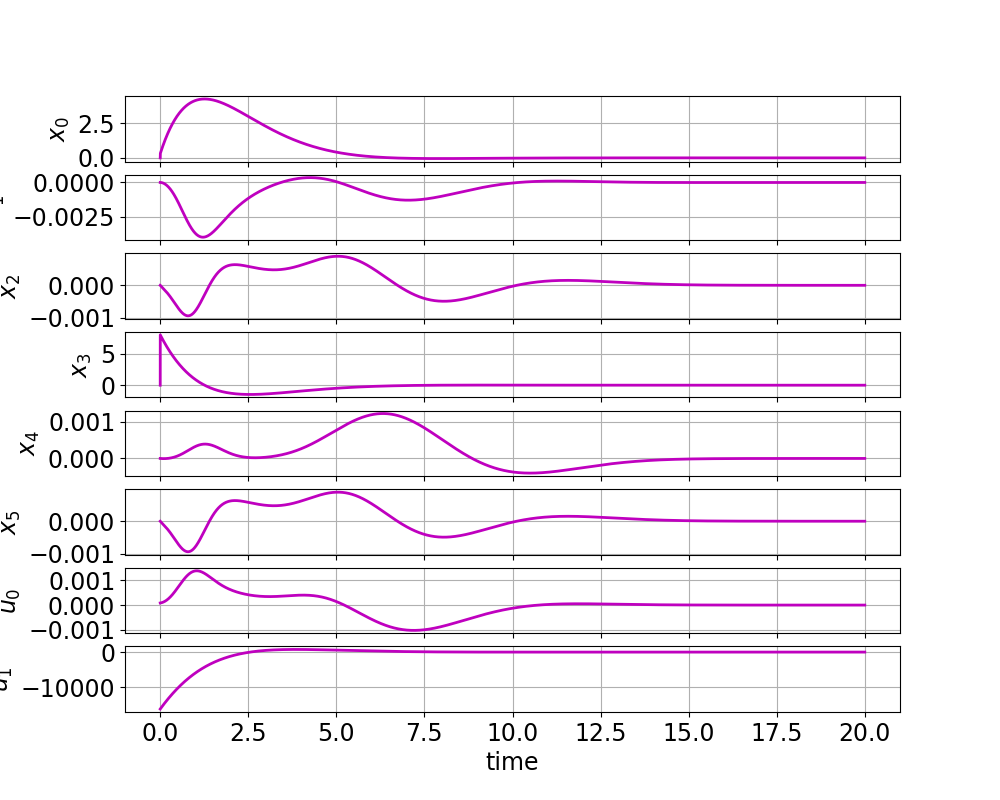
\includegraphics[scale=.50]{Report_OPTCON_Project/figs/Task3/error.png} \\
    \caption{Error}
    \label{fig:error_task3}
\end{figure}
\newpage


%%%%%%%%%% Task 4 %%%%%%%%%%
\chapter{Task 4 - Trajectory tracking via MPC}
Linearizing the vehicle dynamics about the (optimal) trajectory $(x^{opt}, u^{opt})$ computed in Task 2 (chapter \ref{chapter:task2}), exploit an MPC algorithm to track this reference trajectory.

\section{Model Predictive Control}
MPC (Model Predictive Control) is a method that predicts the future behavior of the system and computes an optimal control input to minimize a predefined cost function, taking into account constraints on the system. At periodic intervals, MPC iteratively recomputes the optimal control input based on updated information, allowing for precise and responsive control over time.\\\\
The operation of MPC is as follows:

For each t: 
\begin{itemize}
    \item Measure the current state $x_t$
    \item Compute the optimal trajectory $x*_{t|t}, ..., x*_{t+T|t}, u*_{t|t}, ..., u*_{t+T-1|t}$ with initial condition $x_{t}^{meas}$
    \item Apply the first control input $u*_{t|t}$
    \item Measure $x_{t+1}$ and repeat
\end{itemize}
\begin{figure}[h]
    \centering
    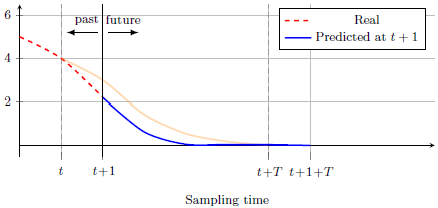
\includegraphics[scale=1.3]{Report_OPTCON_Project/figs/Task4/mpc.png} \\
    \caption{Model Predictive Control}
    \label{fig:enter-label}
\end{figure}
\newpage
\section{Linear Quadratic Case}
Consider the case where the dynamics is linear and the cost quadratic. 
At each time t, with initial measured state $x_t^{meas}$, solve the LQ problem.
\begin{center}
    \min_{x_1, ...,x_{t+T}\atop u_1, ..., u_{t+T-1}} \sum_{\tau=t}^{t+T-1}x_{\tau}^TQx_{\tau}+u_{\tau}^TR_{\tau}u_{\tau}+x_{\tau+T}^T Q_T x_{\tau+T}\\
    \text{subject to} x_{\tau+1}=A_{\tau}x_{\tau}+B_{\tau}u_{\tau} \;\forall\tau=t,\dots,t+T-1\\
    x_t=x_t^{meas}\\
\end{center}
where:
\begin{itemize}
    \item T is the prediction horizon
    \item $x_{\tau}\in\mathbb{R}^n$ and $u_{\tau}\in\mathbb{R}^m$
    \item $A_{\tau}\in\mathbb{R}^{nxn}$ and $B_{\tau}\in\mathbb{R}^{nxm}$ is the prediction model
    \item $Q_{\tau}\in\mathbb{R}^{nxn}$ and $Q_{\tau}=Q_{\tau}^T>=0\;\forall\tau$
    \item $R_{\tau}\in\mathbb{R}^{mxm}$ and $R_{\tau}=R_{\tau}^T>0 \;\forall\tau$
    \item $Q_T\in\mathbb{R}^{nxn}$ and $Q_T=Q_T^T>=0$
\end{itemize}

\section{Tracking of the Optimal Trajectory}
The goal is to track the optimal trajectory through Model Predictive Control, therefore, the cost function to minimize is the one in which $x_{\tau}$ and $u_{\tau}$ represent the errors between the predicted trajectory $(x^{mpc},u^{mpc})$ and optimal one $(x^{mpc},u^{mpc})$.
\\\\
The considered LQ problem is, consequently, as follows:
\begin{align*}
    \min_{x_1, ...,x_{t+T}\atop u_1, ..., u_{t+T-1}} 
    \sum_{\tau=t}^{t+T-1}(x_{\tau}^{mpc}-x_{\tau}^{opt})^TQ_{\tau}(x_{\tau}^{mpc}-x_{\tau}^{opt})+
    &\\+(u_{\tau}^{mpc}-u_{\tau}^{opt})^TR_{\tau}(u_{\tau}^{mpc}-u_{\tau}^{opt})+\;
    &\\+(x_{t+T}^{mpc}-x_{t+T}^{opt})^T Q_T (x_{t+T}^{mpc}-x_{t+T}^{opt})
\end{align*}
\begin{align*}
    \text{subject to} \;(x_{\tau+1}^{mpc}-x_{\tau+1}^{opt})=A_{\tau}(x_{\tau}^{mpc}-x_{\tau}^{opt})+&B_{\tau}(u_{\tau}^{mpc}-u_{\tau}^{opt})\\
    &\forall\tau=t,\dots,t+T-1\\
    (x_{t}^{mpc}-x_{t}^{opt})=(x_t^{meas}-x_t^{opt})
    \end{align*}

\subsection{Costs definition}
The matrices representing the costs, as shown below, have been kept identical to those used in Task 2 (chapter \ref{chapter:task2}), as the significance associated with the state and input elements remains unchanged.
\begin{center}
    $Q_t$ = \begin{bmatrix}
                100 & 0 & 0 & 0 & 0 & 0\\
                0 & 1000 & 0 & 0 & 0 & 0\\
                0 & 0 & 10 & 0 & 0 & 0\\
                0 & 0 & 0 & 100 & 0 & 0\\
                0 & 0 & 0 & 0 & 100 & 0\\
                0 & 0 & 0 & 0 & 0 & 10\\
            \end{bmatrix}
    $R_t$ = \begin{bmatrix}
                10000 & 0\\
                0 & 0.0001\\
            \end{bmatrix}
\end{center}
\begin{center}
$Q_T$ = solution of Riccati equation
\end{center}

\newpage
\section{Results}
Following, the plot of the MPC trajectory in relation to the desired optimal trajectory for all states and inputs can be observed.
\begin{figure}[h]
    \centering
    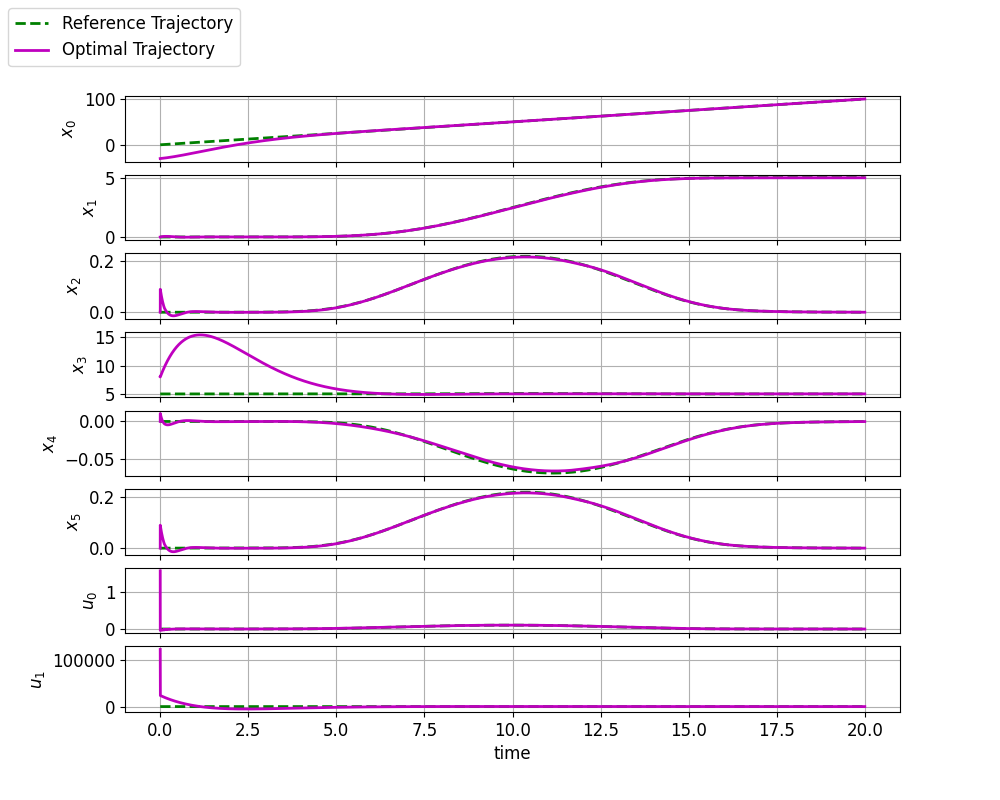
\includegraphics[scale=.40]{figs/Task4/opt_trajectory} \\
    \caption{Optimal Trajectory}
    \label{fig:enter-label}
\end{figure}
\newpage
\\
Given the perturbed inputs as follows: 
\begin{center}
    $x_0=[-30, 0, 0, 8, 0, 0]^T$
\end{center}
the following plot shows the tracking error for different initial conditions.
\begin{figure}[h]
    \centering
    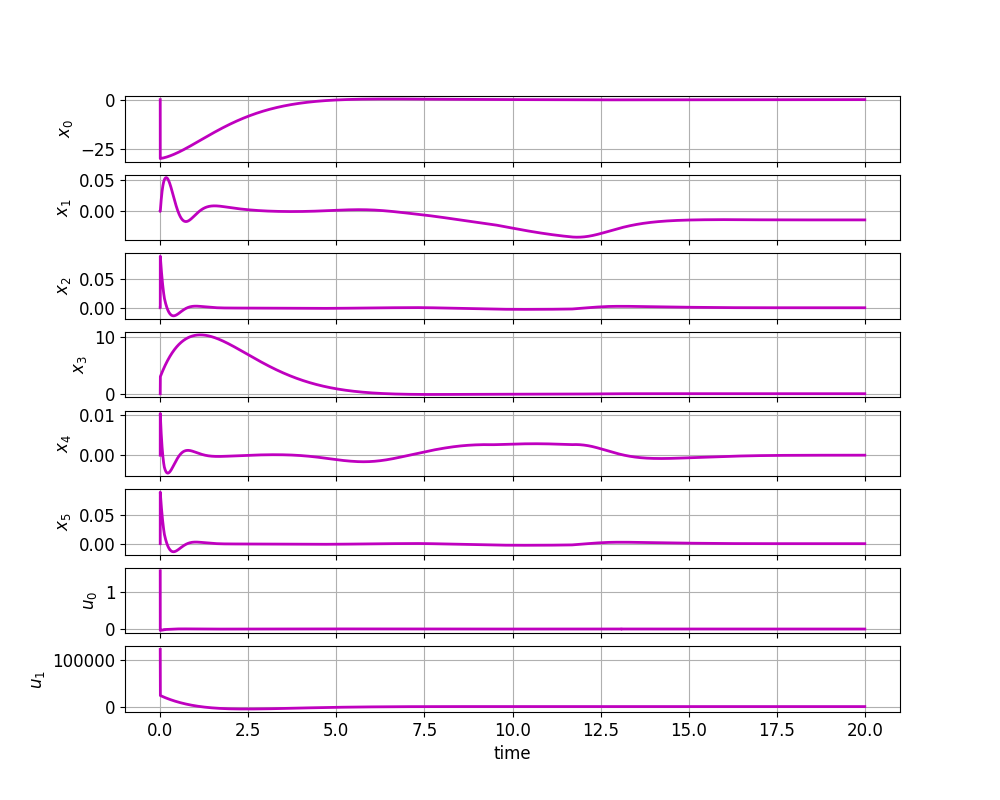
\includegraphics[scale=.40]{figs/Task4/error} \\
    \caption{Error}
    \label{fig:enter-label}
\end{figure}

\newpage
%%%%%%%%%% Task 5 %%%%%%%%%%
\chapter{Task 5 - Animation}

Produce a simple animation of the vehicle executing Task 3 (chapter \ref{chapter:task3}).

\section{Results}
Given the optimal trajectories obtained in the computation of Task 3 (\ref{chapter:task3}), the animation was implemented using Python. Below, snapshots of the animation are presented.
\begin{figure}[h]
    \centering
    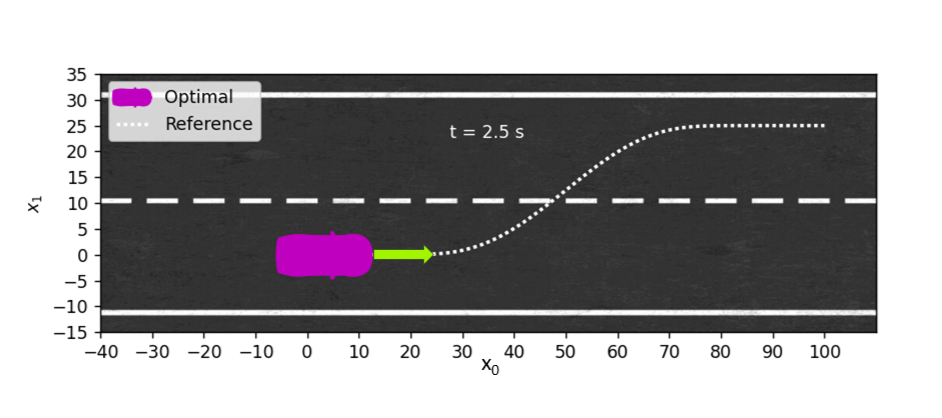
\includegraphics[scale=.60]{figs/Task5/Vehicle_2.5s} \\
    \caption{Animation of the vehicle at t=2.5}
    \label{fig:enter-label}
\end{figure}

\begin{figure}[h]
    \centering
    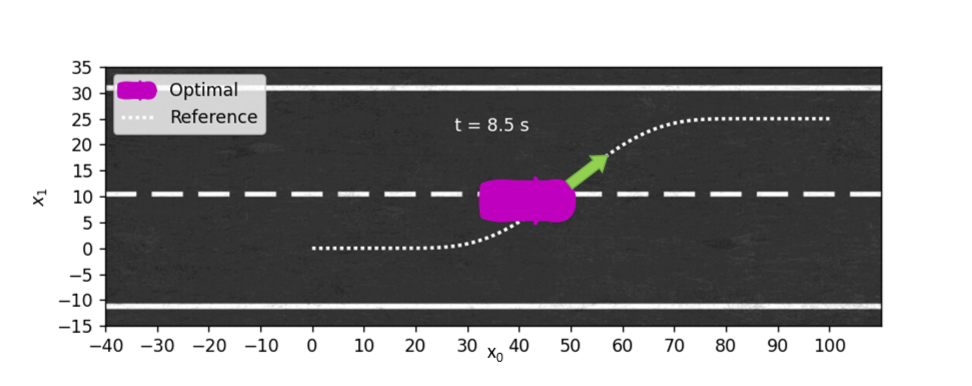
\includegraphics[scale=.60]{figs/Task5/Vehicle_8.5s} \\
    \caption{Animation of the vehicle at t=8.5}
    \label{fig:enter-label}
\end{figure}
\begin{figure}[h]
    \centering
    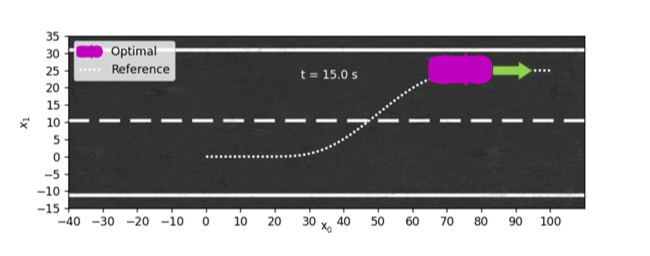
\includegraphics[scale=.90]{figs/Task5/Vehicle_15s} \\
    \caption{Animation of the vehicle at t=15}
    \label{fig:enter-label}
\end{figure}
%%%%%%%%%% Conclusions %%%%%%%%%%
\chapter*{Conclusions}
\addcontentsline{toc}{chapter}{Conclusions}
Through the successful execution of this project, various objectives were addressed, leading to the development of an optimal control system for a simple bicycle model with static load transfer for an autonomous vehicle. The project milestones include:
\begin{itemize}
    \item \textbf{Task 0 - Problem setup}: discretization of the vehicle dynamics, writing of the discrete-time state-space equations and implementation of the dynamics function;
    \item \textbf{Task 1 - Trajectory Generation (I)}: Implemented a Newton-like algorithm to craft an optimal trajectory enabling the autonomous vehicle to smoothly transition from one equilibrium configuration to another. The Armijo algorithm was utilized for step size selection;
    \item \textbf{Task 2 - Trajectory Generation (II)}: Employed the Newton-like algorithm once more to formulate an optimal trajectory between two equilibria, incorporating a reference curve designed as a sigmoid function;
    \item \textbf{Task 3 - Trajectory Tracking via LQR}: Utilized the Linear Quadratic Regulator (LQR) method to track the optimal trajectory designed in Task 2. Additionally, demonstrated the controller's efficacy in reaching the target even when initiated from perturbed initial conditions;
    \item \textbf{Task 4 - Trajectory Tracking via MPC}: Applied the Model Predictive Control (MPC) algorithm to follow the optimal trajectory crafted in Task 2. Once again, substantiated the controller's ability to attain the target despite perturbed initial conditions.
\end{itemize}

%%%%%%%%%%%%%%%%%%%%%%%%%%%%%%%%%%%%%%

\end{document}